%%%%%
%%%%% Supporting material for Sandwich paper.
%%%%% Compile with pdflatex as figures are not eps.
%%%%%
\documentclass[12pt,twoside]{article}
\usepackage{graphicx}

\setlength{\hoffset}{-1in}
\setlength{\voffset}{-1in}

\setlength{\topmargin}{2cm}
\setlength{\evensidemargin}{3.1cm}
\setlength{\oddsidemargin}{3.1cm}

\setlength{\textwidth}{14.8cm}
\setlength{\textheight}{23cm}

\setlength{\parindent}{0pt}
\setlength{\parskip}{\medskipamount}
\pagestyle{empty}


\begin{document}


{\bf Supplementary Information for: Self-assembly of colloid-cholesteric
composites: A route to switchable optical materials}

Here, we give more details of the simulation method, protocol, and parameters used. We also provide additional figures complementing the main text, and discuss the matching of simulation units to physical units. 

{\bf 1. Thermodynamics}

The thermodynamics of the cholesteric liquid crystal can be described
by means of a  Landau-de Gennes free energy functional $\cal F$,
whose density is written as $f$:
\begin{eqnarray}
{\cal F}[{\bf Q}]&=&\int d^3{\bf r} f({\bf Q}({\bf r})).
\end{eqnarray}
This free energy density $f = f({\bf Q})$ may be expanded in powers of the
order parameter ${\bf Q}$ and its gradients; ${\bf Q}$ is a traceless 
and symmetric tensor which we will denote from now on in subscript
notation as $Q_{\alpha\beta}$.
The largest eigenvalue $q$ and corresponding eigenvector $n_\alpha$
of $Q_{\alpha\beta}$ describe the local strength and major orientation axis
of molecular order.
The theory based on the tensor $Q_{\alpha\beta}$, rather than a theory based
solely
on the director field $n_\alpha ({\bf r})$, allows treatment of disclinations
(defect lines) in whose cores $n_\alpha$ is undefined.

Explicitly, the free energy density is:
\begin{eqnarray}
f(Q_{\alpha\beta}) &=& {\textstyle \frac{1}{2}} A_0
 \left(1- {\textstyle \frac{1}{3}}\gamma \right)Q^2_{\alpha \beta}
-{\textstyle \frac{1}{3}}A_0\gamma Q_{\alpha \beta} Q_{\beta \gamma}Q_{\gamma \alpha} 
+ {\textstyle \frac{1}{4}} A_0\gamma (Q^2_{\alpha \beta})^2  \nonumber\\
&+& {\textstyle \frac{1}{2}} K(\varepsilon_{\alpha \gamma \delta}
\partial_\gamma Q_{\delta \beta} + 2 q_0 Q_{\alpha \beta})^2
+ {\textstyle \frac{1}{2}} K (\partial_\beta Q_{\alpha \beta})^2.
\label{free}
\end{eqnarray}
Here, repeated indices are summed over, while terms of the form
$Q^2_{\alpha\beta}$ should be expanded to read $Q_{\alpha\beta}Q_{\alpha\beta}$;
$\varepsilon_{\alpha\gamma\delta}$ is the permutation tensor.
The first three terms are a bulk free energy density whose overall scale
is set by $A_0$ (discussed further below); $\gamma$ is a control parameter
related to a reduced temperature. Varying the latter in the absence of
chiral terms ($q_0=0$) gives an isotropic-nematic transition at
$\gamma = 2.7$ with a mean-field spinodal instability at $\gamma = 3$.

The remaining two terms of the free energy density in Eq.~\ref{free} describe
distortions of the order parameter field. In theoretical work and when
describing a generic rather than a specific system, it is 
conventional~\cite{blue1,deGennes} to
assume that splay, bend and twist deformations of the director are equally
costly, that is, there is a single elastic constant $K$. The parameter $q_0$
is related to the helical pitch length $p$ via $q_0=2\pi/p$,
describing one full turn of the director in the cholesteric phase.

There are two dimensionless numbers, which are commonly referred to as
$\kappa$, the chirality, and  $\tau$, the reduced temperature
\cite{blue1} which can be used to characterise the system. In terms of
the parameters in the free energy density, these are:
\begin{eqnarray}\label{cntrl-param} 
\tau&=&\frac{27(1-\gamma/3)}{\gamma}\label{tau}\\
\kappa&=&\sqrt{\frac{108\ K\, q_0^2}{A_0\, \gamma}}\label{kappa}.
\end{eqnarray}
If the free energy density Eq.~\ref{free} is made dimensionless, $\tau$
appears as prefactor of the term  quadratic in $Q_{\alpha\beta}$,
whereas $\kappa$
quantifies the ratio between bulk and  gradient free energy terms. The
chirality and reduced temperature may be used to characterise an equilibrium
phase diagram of the blue phases in bulk cholesteric liquid crystals
\cite{blue1,oliver1}.

The effect of an electric field can be modelled by including the following
term in the bulk free energy density:
\begin{equation}
-\frac{\epsilon_a}{12\pi} E_{\alpha}Q_{\alpha\beta}E_{\beta},
\end{equation} 
where $E_{\alpha}$ are the components of the electric field, and 
$\epsilon_a$ (here assumed positive) is the dielectric anisotropy of the liquid
crystal. The strength of the electric field is quantified via
one further dimensionless number
\begin{equation}
{\cal E}^2 = \frac{27 \epsilon_a}{32 \pi A_0 \gamma} E_\alpha E_\alpha.
\end{equation}
The quantity ${\cal E}$ will be referred to as the reduced field strength.

{\bf 1.1 Surface free energy}

In addition to the fluid free energy density $f(Q_{\alpha\beta})$, a surface
free energy density is also present to represent the energetic cost of
anchoring at a solid surface. If the preferred order parameter tensor
at the solid surface is $Q^0_{\alpha\beta}$, then the surface free energy
density (per unit area) is
\begin{equation}
f_s(Q_{\alpha\beta}, Q^0_{\alpha\beta})
= {\textstyle \frac{1}{2}}W(Q_{\alpha\beta} - Q^0_{\alpha\beta})^2,
\end{equation}
where $W$ is a constant determining the strength of the anchoring.
The determination of $Q^0_{\alpha\beta}$ for normal and planar anchoring is
discussed below. For a colloid of radius $R$, the strength of the surface
anchoring compared which the bulk fluid elastic constant may be quantified
by the dimensionless parameter $WR/K$. For small values of this parameter,
the presence of a colloid surface should have little impact on the local
fluid LC ordering.

% NO REDSHIFT

{\bf 2. Dynamics}

{\bf 2.1 Order parameter}

A framework for the dynamics of liquid crystals is provided by the 
Beris-Edwards model \cite{beris}, in which the time evolution of the
tensor order parameter obeys
\begin{equation}
\label{eom}
\left(\partial_t+ u_\nu \partial_\nu \right) Q_{\alpha\beta} - S_{\alpha\beta}
= \Gamma H_{\alpha\beta}.
\end{equation}
In the absence of flow, Eq.~\ref{eom} describes a relaxation towards
equilibrium on a timescale determined by a collective rotational diffusion 
constant $\Gamma$. This relaxation is driven by the molecular field
$H_{\alpha\beta}$, which is the functional derivative of the free energy
with respect to the order parameter \cite{beris}:
\begin{equation}
H_{\alpha\beta} = -\frac{\delta {\cal F}} {\delta Q_{\alpha\beta}} 
+ {\textstyle \frac{1}{3}} \delta_{\alpha\beta} 
\mathrm{Tr}\left(\frac{\delta {\cal F}}{\delta Q_{\alpha\beta}}\right).
\end{equation}

The tensor $S_{\alpha\beta}$ in Eq.~\ref{eom} completes the material
derivative for rod-like molecules \cite{beris}. It couples the order
parameter to the symmetric and antisymmetric parts of the velocity 
gradient tensor $W_{\alpha \beta}\equiv\partial_\beta u_\alpha$.
The symmetric part $A_{\alpha\beta}$ and the antisymmetric part
$\Omega_{\alpha\beta}$ are defined as 
\begin{equation}
A_{\alpha\beta} = {\textstyle \frac{1}{2}} (W_{\alpha\beta} + W_{\beta\alpha}),
\end{equation}
and
\begin{equation}
\Omega_{\alpha\beta} = {\textstyle \frac{1}{2}} (W_{\alpha\beta} - W_{\beta\alpha}).
\end{equation}
This full coupling term is then
\begin{eqnarray}
\label{coupling-term}
S_{\alpha\beta}  &=&
(\xi A_{\alpha\nu} + \Omega_{\alpha\nu})
(Q_{\nu\beta} + {\textstyle \frac{1}{3}}\delta_{\nu\beta})
+
(Q_{\alpha\nu} + {\textstyle \frac{1}{3}} \delta_{\alpha\nu})
(\xi A_{\nu\beta} - \Omega_{\nu\beta})
\nonumber\\ 
&-&2 \xi ({Q_{\alpha\beta} + {\textstyle \frac{1}{3}}\delta_{\alpha\beta}})
Q_{\nu\nu} W_{\nu\nu}.
\end{eqnarray}
%CORRECT TRACE?!
Here, $\xi$ is a material-dependent that controls the
relative importance of rotational and elongational flow for molecular
alignment, and determines in practice how the orientational order
responds to a local shear flow. 
In all cases, the value used here is $\xi = 0.7$, which is within
the `flow aligning' regime, where molecules align at a fixed angle
(the Leslie angle) to the flow direction in weak simple shear \cite{deGennes}.
The value of the collective rotational diffusion used in all simulations is
$\Gamma = 0.5$ in simulation units.

{\bf 2.2 Hydrodynamics}

The momentum evolution obeys a Navier-Stokes equation driven by the divergence
of a generalised stress $P_{\alpha\beta}$:
\begin{equation}
\label{nse}
\rho\,\partial_tu_\alpha +\rho \,u_\beta \partial_\beta u_\alpha
=\partial_\beta P_{\alpha\beta}.
\end{equation}
The pressure tensor $P_{\alpha\beta}$ is, in general, asymmetric and includes
both viscous and thermodynamic components:
\begin{eqnarray}
P_{\alpha \beta}&=&
- p_0 \delta_{\alpha \beta} 
+ \eta \{ \partial_\alpha u_\beta + \partial_\beta u_\alpha\}
\nonumber\\
&-&  \xi H_{\alpha \gamma}\left(Q_{\gamma \beta}
+ {\textstyle \frac{1}{3}} \delta_{\gamma \beta} \right)
-\xi \left(Q_{\alpha \gamma}
+ { \textstyle \frac{1}{3}} \delta_{\alpha \gamma}\right) H_{\gamma \beta}
\nonumber\\ 
&+& 2 \xi  \left(Q_{\alpha \beta}
+ {\textstyle \frac{1}{3}} \delta_{\alpha \beta}\right) Q_{\gamma \nu} H_{\gamma \nu}
-\partial_\alpha Q_{\gamma \nu}
\frac{\delta{\cal F}}{\delta \partial_{\beta} Q_{\gamma \nu}}\nonumber\\
&+& Q_{\alpha \gamma}H_{\gamma \beta}-H_{\alpha \gamma} Q_{\gamma \beta}.
\end{eqnarray}
A lattice Boltzmann flow solver is used, where the isotropic pressure $p_0$
and viscous terms are managed directly by the solver (as in a simple Newtonian
fluid, of viscosity $\eta$), whereas the divergence of the remaining terms
is treated as a local force density on the fluid. In all simulations
reported the mean fluid density $\rho = 1$ and the viscosity
$\eta = 0.01$ (simulations in confined geometry also used enhanced
bulk viscosity $\zeta = 10\eta$ to ensure numerical stability).


{\bf 3. Surface boundary conditions}

Hydrodynamic boundary conditions for solid objects are handled via
the lattice Boltzmann solver. In particular, the standard method of
bounce-back on links is used for both colloids and confining walls
\cite{ladd94,nguyen2002}. Boundary conditions for the order parameter
are set out in \cite{juho}.

{\bf 3.1 Colloids}

In all the simulations reported here the preferred orientation of the
director field at the colloid surface is normal to the surface. The
required nematic director at the particle surface in a given location
$\hat{n}^0_\alpha$ may then be determined from geometry alone,
and a preferred order parameter $Q_{\alpha\beta}^0$ is computed via
\begin{equation}
Q^0_{\alpha\beta} = q^0(\hat{n}_\alpha^0 \hat{n}_\beta^0 
- {\textstyle \frac{1}{3}} \delta_{\alpha\beta}).
\label{eq:surf_q}
\end{equation}
The magnitude of surface order $q^0$ is set by
\begin{equation}
q^0 = {\textstyle \frac{2}{3}} \left( {\textstyle \frac{1}{4}} 
+ {\textstyle \frac{3}{4}} \sqrt{1 + (8/3\gamma)} \right)
\label{eq:surf_q0}
\end{equation}
which corresponds to the bulk order in a defect-free nematically ordered 
sample~\cite{denniston} (this is also very close to the value of the order 
parameter in a cholesteric or in a blue phase away from disclinations).

In all simulations the colloidal (hard sphere) radius is $R = 2.3$. To
prevent colloids overlapping at the hard sphere radius, an additional
short range soft potential is included. This takes the form of
$V(h) = \epsilon (\sigma/h)$ where $h$ is the surface to surface separation.
The parameters are $\epsilon = 0.0004$ and $\sigma = 0.1$ in simulation
units. Both potential and resulting force are smoothly matched to zero at
a cut-off distance of $h_c = 0.25$ simulation units.

{\bf 3.2 Confining walls}

The confining solid walls, which are flat and stationary, have the
same normal boundary condition as at colloid surface. In addition,
degenerate planar anchoring is applied at the walls, where the
preferred nematic director may adopt any orientation parallel
to the surface. The preferred direction is determined explicitly
by projecting the local fluid order parameter to the plane of the
wall \cite{fournier2005}. Eq.~\ref{eq:surf_q} and Eq.~\ref{eq:surf_q0}
are then used as before.

To prevent the colloids being forced into the wall, a correction
to the lubrication force on the colloid is added for very low colloid
surface to wall surface separations $h < 0.5$ lattice spacing. The
correction is based on the analytic expression for the lubrication
between a sphere and a flat surface.

{\bf 4. Protocol and parameter details}

{\bf 4.1 Bulk blue phase I}

The parameters for the free energy are chosen to be representative
of blue phase I: chirality $\kappa \sim 0.7$ and reduced temperature
$\tau = -0.25$.
The full free energy parameters are shown in Table~\ref{table:params}.
The order parameter tensor $Q_{\alpha\beta}$ for bulk blue phase I is
initialised from an approximation in high chirality limit
\cite{blue1,oliver1}. Systems of 128$^3$ lattice sites are
used with a pitch length of $p = 32\sqrt{2}$, which accommodates 4$^3$
unit cells with fully periodic boundary conditions.
Simulations at different solid volume fractions (1\% and 4\%), and different 
surface anchoring strengths ($WR/K = 0.23$ and $WR/K = 2.3$) representing
``weak'' and ``strong'' anchoring are run for two million simulation
time steps.
The initial distribution of the colloid positions is set at random
for the required solid volume fraction; the colloids are initially
at rest.

To generate a disordered network of disclination lines, a ``quench''
is performed in which the order parameter is initialised via a
locally chosen random director, and
Eq.~\ref{eq:surf_q} employed with a small amplitude $q^0 = 10^{-7}$ to
provide an order parameter.
We avoid the mean-field spinodal point at $\gamma = 3.0$:
the parameters are the same as for the initial simulations with
pitch $p = 32\sqrt{2}$. The chirality and reduced temperature (see
Table~\ref{table:params}) remain appropriate for BPI.
Colloids are added as before and the simulations run for 2 million
simulation steps.

For simplicity, we do not allow the size of the BPI unit cell to 
dynamically readjust to minimize free energy (there is no 
``redshift''~\cite{blue1}): this would lead to quantitatively different 
values of the free energy, but qualitatively similar structures. 

{\bf 4.2 Confined blue phase I}

Here, a narrow sandwich of fluid is placed between flat walls in
perpendicular to the narrow coordinate direction, and with periodic
boundaries in the other two directions. The system size used in all
cases is 256$^2 \times$56 lattice sites. Each simulation is a ``quench''
in a similar manner to that used in the bulk: the order parameter is
initialised randomly. The free energy parameters (see Table~\ref{table:params})
are again appropriate for (equilibrium) blue phase I
(chirality $\kappa = 0.8$ and
reduced temperature $\tau = -0.25$). The cholesteric pitch is set
to be $p = 64$, providing a slightly better resolution than the bulk
simulations.

The surface anchoring for colloids is as before: always normal, but with
$WR/K = 0.23$ and $WR/K = 2.3$. The colloid solid volume fractions are
1\% and 4\%. Wall anchoring is either normal or planar with $W/K = 1$
in simulation units. All simulations are run for two million simulation
time steps.

{\bf 4.3 External electric field}

For the simulations of BPIII with colloidal particles a system size of
$128^3$ is used with a cholesteric pitch of $p=32$ in lattice units. 
The simulations are
performed at chirality $\kappa=2.6$ and reduced temperature $\tau=-0.25$.  
An initial configuration of
randomly oriented and positioned double twist cylinders is used,
from which an amorphous BPIII network emerges \cite{oliver-bp3}. This structure
is equilibrated for $6\times10^{5}$ LB time steps until no significant
further evolution is observed. 

The colloidal particles with weak
normal anchoring ($WR / K= 0.23$), are then inserted with randomly chosen positions,
and the composite system is equilibrated for another $1.2\times10^{6}$
time steps.
At the end of the equilibration phase the uniform electric field
with reduced field strength ${\cal E} = 0.8$ 
is switched on (oriented along the $z$-direction), and the simulation
run for a further $1.2\times10^{6}$ time steps.
This is found to be sufficiently long for a hexagonal structure to
emerge and saturate.
If the electric field is then switched off, and the system quickly relaxes
to a metastable state which shows a residual anisotropy in the
colloidal distribution. The total length of this final relaxation phase
is $1\times10^6$ LB time steps.

\begin{table}[h]
\begin{center}
\begin{tabular}{|l|c|c|c|c|c|c|c|}
\hline
         & $A_0$ & $\gamma$ & $K$ & $p$ & $\kappa$ & $\tau$ & $WR/K$\\
\hline 
Bulk BPI & 0.01 & 3.086 & 0.007061 & 32$\sqrt{2}$ & 0.6902 & -0.2500 &
0.23, 2.3\\
\hline
Bulk Quench & 0.01 & 3.086 & 0.007061 & 32$\sqrt{2}$ & 0.6902 & -0.2500 &
0.23, 2.3 \\
\hline
Confined & 0.01 & 3.086 & 0.01897 & 64 & 0.8 & -0.2500 & 0.23, 2.3\\
\hline
External field & 0.004& 3.086 & 0.02 & 32 & 2.6 & -0.2500 & 0.23\\ 
\hline
\end{tabular}
\end{center}
\caption{Free energy parameters used in the simulations. Bulk BPI
correspond to Fig.~1 (A-D), bulk quench to Fig.~1 (E--H); confined
geometries are shown in Fig.~2; and the external field case is
relevant for Fig.~3.}
\label{table:params}
\end{table}

{\bf 4.4 Disclination rendering}

In all cases visualisation of the defect lines is carried out via
an isosurface of the scalar order parameter $q$ determined from the
largest eigenvalue of the local order parameter tensor. A low value
of the scalar order parameter $q$ (typically in the range 0.12--0.14)
unambiguously identifies the disclinations.

{\bf 4.4 Computation of the structure factor}

In order to demonstrate structural information about the field-aligned 
states and the residual anisotropy after switch off we followed a 
procedure similar to the one described in \cite{oliver-bp3}.
The structure factor in the current approach is defined via
the Fourier transform of the colloid density:

\begin{eqnarray}
S({\bf k})&=&|F({\bf k})|^2\\
F({\bf k})&=&\int_V d{\bf r} \rho({\bf r}) e^{i {\bf k r}}
\end{eqnarray}

The colloid density $\rho({\bf r})$ is a discretised density and taken to be
$\rho({\bf r})=1$ if a lattice site at ${\bf r}$ is part of a colloid
and $\rho({\bf r})=0$ otherwise. This definition, which deviates from the 
standard definition of a structure factor and does not consider the colloids 
as pointlike objects, allows to gain the same structural information
in a simpler way.

{\bf 5. Parameter mapping to physical units}

To get from simulation to physical units, a calibration of scales of
length, energy and time in the simulations is required. For similar
mappings see,
e.g.~\cite{denniston2}.

The length scale can be set by mapping the half pitch to a realistic blue
phase unit cell size, which is in the 100--500~nm range \cite{blue1}. 
For bulk simulations (Fig.~1 and Fig.~3 in the main text), a suitable choice
is one where one simulation unit (lattice site) corresponds to 10~nm. Therefore
the colloidal size in Figs.~1 and~3 corresponds to $\sim$ 50~nm. 

To obtain an energy scale, it is possible to choose $A_0 \simeq 10^6$~Pa,
which is reasonable following Ref.~\cite{blue1} (this is also the choice in
Ref.~\cite{oliver2}). This choice leads to a simulation unit of
free energy (or stress) equal to $10^{8}$~Pa in Figs.~1 and~3.
From the energy and length scales one can map elastic constants to
physical units: for instance, the simulation in Fig.~1 corresponds to
a liquid crystal with splay, bend and twist (Frank) elastic constants
equal to 35 pN (or equivalently $K=70$~pN).

The timescale calibration may be obtained from (see e.g.~\cite{denniston})
\begin{equation}
\gamma_1=\frac{2q^2}{\Gamma},
\end{equation}
which relates the rotational viscosity $\gamma_1$ to the ordering strength
$q$ and the order parameter mobility $\Gamma$.
In the present simulations, $\Gamma = 0.5$ and the value of $\gamma$
for the simulation in Fig.~1 leads to $q=1/2$.   
For real liquid crystalline materials, $\gamma_1$ usually lies in range
$10^{-2}-1$ Pa s~\cite{deGennes}; for definiteness say
$\gamma_1 = 1$~Pa~s (equivalently 10 poise). Given the previous mapping for
free energy (or stress) units, this leads to a simulation unit of time equal
to $10^{-8}$~s. The total simulated time in Figs. 1-3 is therefore in the
millisecond range. 

To calibrate the electric field strength 
one can equate the value of the dimensionless parameter ${\cal E}$ in the 
simulations with that of a hypothetical experiment.
Given the previous value for $A_0$, and a dielectric anisotropy of 20
(or equivalently $\epsilon_a=20\epsilon_0$, with $\epsilon_0$ the
dielectric permittivity of vacuum), an electric field
of 100 V/$\mu$m is obtained. This corresponds to a value of
${\cal E}\sim 0.4$ (considering a value of $\gamma=3.0857$ as in
Fig.~3 of the main text).

Given these mappings, all quantities can be easily transformed from
simulation to physical units and vice versa. For example Figs.~1 and~2
use an isotropic viscosity $\eta \simeq$~0.01 and~0.1 in simulation units,
which translate into $0.01-0.1$~Pa~s respectively. This is sensible (if 
slightly low) for a molecular nematogen in the isotropic phase. 
The effective viscosity in ordered phases is higher, but this is ensured
in our model by the coupling to the order parameter.
Note that the density is set to unity in the simulations: this
corresponds to a fluid density which is about a thousand times larger
than in experiments. This makes no difference in practice as
the Reynolds number $= \rho V\Lambda/\eta$ (where $V$ is a typical
velocity, in our simulations around $10^{-5}$ in lattice units, 
and $\Lambda$ is a typical length scale, e.g. the size of a unit cell) 
remains small enough~\cite{codef}. 

To summarize, the simulations represent BP-forming materials, with the
interpretation of the simulation units for length, time, and energy
density being close to 10~nm, 10~ns, and 100~MPa respectively.

%ISSUE: Temperature?  Temperature: $T = 2.133333 10^{-9}$ CHECK

\vfill
\pagebreak


\begin{thebibliography}{99}

\bibitem{blue1}
D.C. Wright and N.D. Mermin,
%  Crystalline liquids -- the blue phases.
{\it Rev. Mod. Phys.} {\bf 61,} 385-432 (1989).
\bibitem{deGennes}
P.-G. de Gennes, J. Prost,
{\it The Physics of Liquid Crystals} (Oxford Univ. Press, New York, 1993).
%\bibitem{marendu1}
%D. Marenduzzo, E.  Orlandini, M. E. Cates, J. M. Yeomans,
%{\rm Steady-state hydrodynamic instabilities of active liquid crystals:
%Hybrid lattice Boltzmann simulations.}
%{\it Phys. Rev. E} {\bf 76}, 031921 (2007).
%\bibitem{marendu2}
%O. Henrich, D. Marenduzzo, K. Stratford, M. E. Cates, 
%{\rm Domain growth in cholesteric blue phases:
%hybrid lattice Boltzmann simulations}.
%{\it Comput. Math. Appl.}, doi:10.1016/j.camwa.2009.08.047[dx.doi.org] (2009).
%\bibitem{marendu3}
%M. E. Cates, O. Henrich, D. Marenduzzo, K. Stratford,
%{\rm  Lattice Boltzmann simulations of liquid crystalline fluids:
%active gels and blue phases.}
%{\it Soft Matter} {\bf 5}, 3791-3800 (2009).
\bibitem{oliver1}
O. Henrich, D. Marenduzzo, K. Stratford, and M.E. Cates,
%Thermodynamics of blue phases in electric fields
\textit{Phys. Rev. E}, \textbf{81} 031706 (2010).
\bibitem{beris}
A. N. Beris, B. J. Edwards, 
{\it Thermodynamics of Flowing Systems with Internal Microstructure}
(Oxford Univ. Press, New York, 1994).
\bibitem{ladd94}
A.J.C. Ladd,
\textit{J. Fluid Mech.} \textbf{271}, 285 (1994); \textit{ibid.} \textbf{271}
311 (1994).
\bibitem{nguyen2002}
N.-Q. Nguyen and A.J.C. Ladd,
\textit{Phys. Rev. E} \textbf{66} 046708 (2002).
\bibitem{juho}
J.S. Lintuvuori, D. Marenduzzo, K. Stratford, and M.E. Cates,
\textit{J. Mater. Chem.} \textbf{20}, 10547 (2010).
\bibitem{denniston}
C. Denniston, E. Orlandini, J. M. Yeomans, 
\textit{Phys. Rev. E} \textbf{63}, 056702 (2001).
\bibitem{fournier2005}
J.-B. Fournier and P. Galatola,
\textit{Europhys. Lett.} \textbf{72}, 403 (2005).
\bibitem{oliver-bp3}
O. Henrich, K. Stratford, M.~E. Cates, D. Marenduzzo,
{\it Phys. Rev. Lett.} {\bf 106}, 107802 (2011).
\bibitem{denniston2}
C. Denniston, D. Marenduzzo, E. Orlandini, J. M.  Yeomans, 
\textit{Philos. Trans. R. Soc. London, Ser. A} \textbf{362}, 1745 (2004).
\bibitem{oliver2}
O. Henrich, K. Stratford, D. Marenduzzo, M. E. Cates, 
\textit{Proc. Acad. Sci. USA} \textbf{107}, 1312 (2010).
\bibitem{codef} M. E. Cates,  et al., 
\textit{J. Phys. Condens. Matter} \textbf{16},  3903 (2004). 


\end{thebibliography}

\vfill\pagebreak


{\bf Supplementry Figures and Animations}

\begin{figure}[!h]
\begin{center}
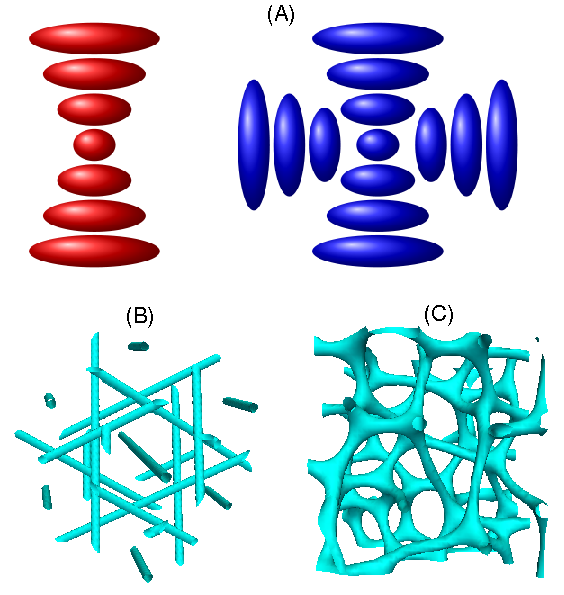
\includegraphics[scale=0.8]{support-fig1.png}
\end{center}
\caption{
(A) Schematic representation of the director field
in a cholesteric (left) and within a double twist cylinder (right).
(B) Snapshot of the disclination network in an equilibrated 
blue phase I structure. (C) Same as (B) for an amorphous blue phase III
network.}
\end{figure}

\newpage

\begin{figure}[!h]
\begin{center}
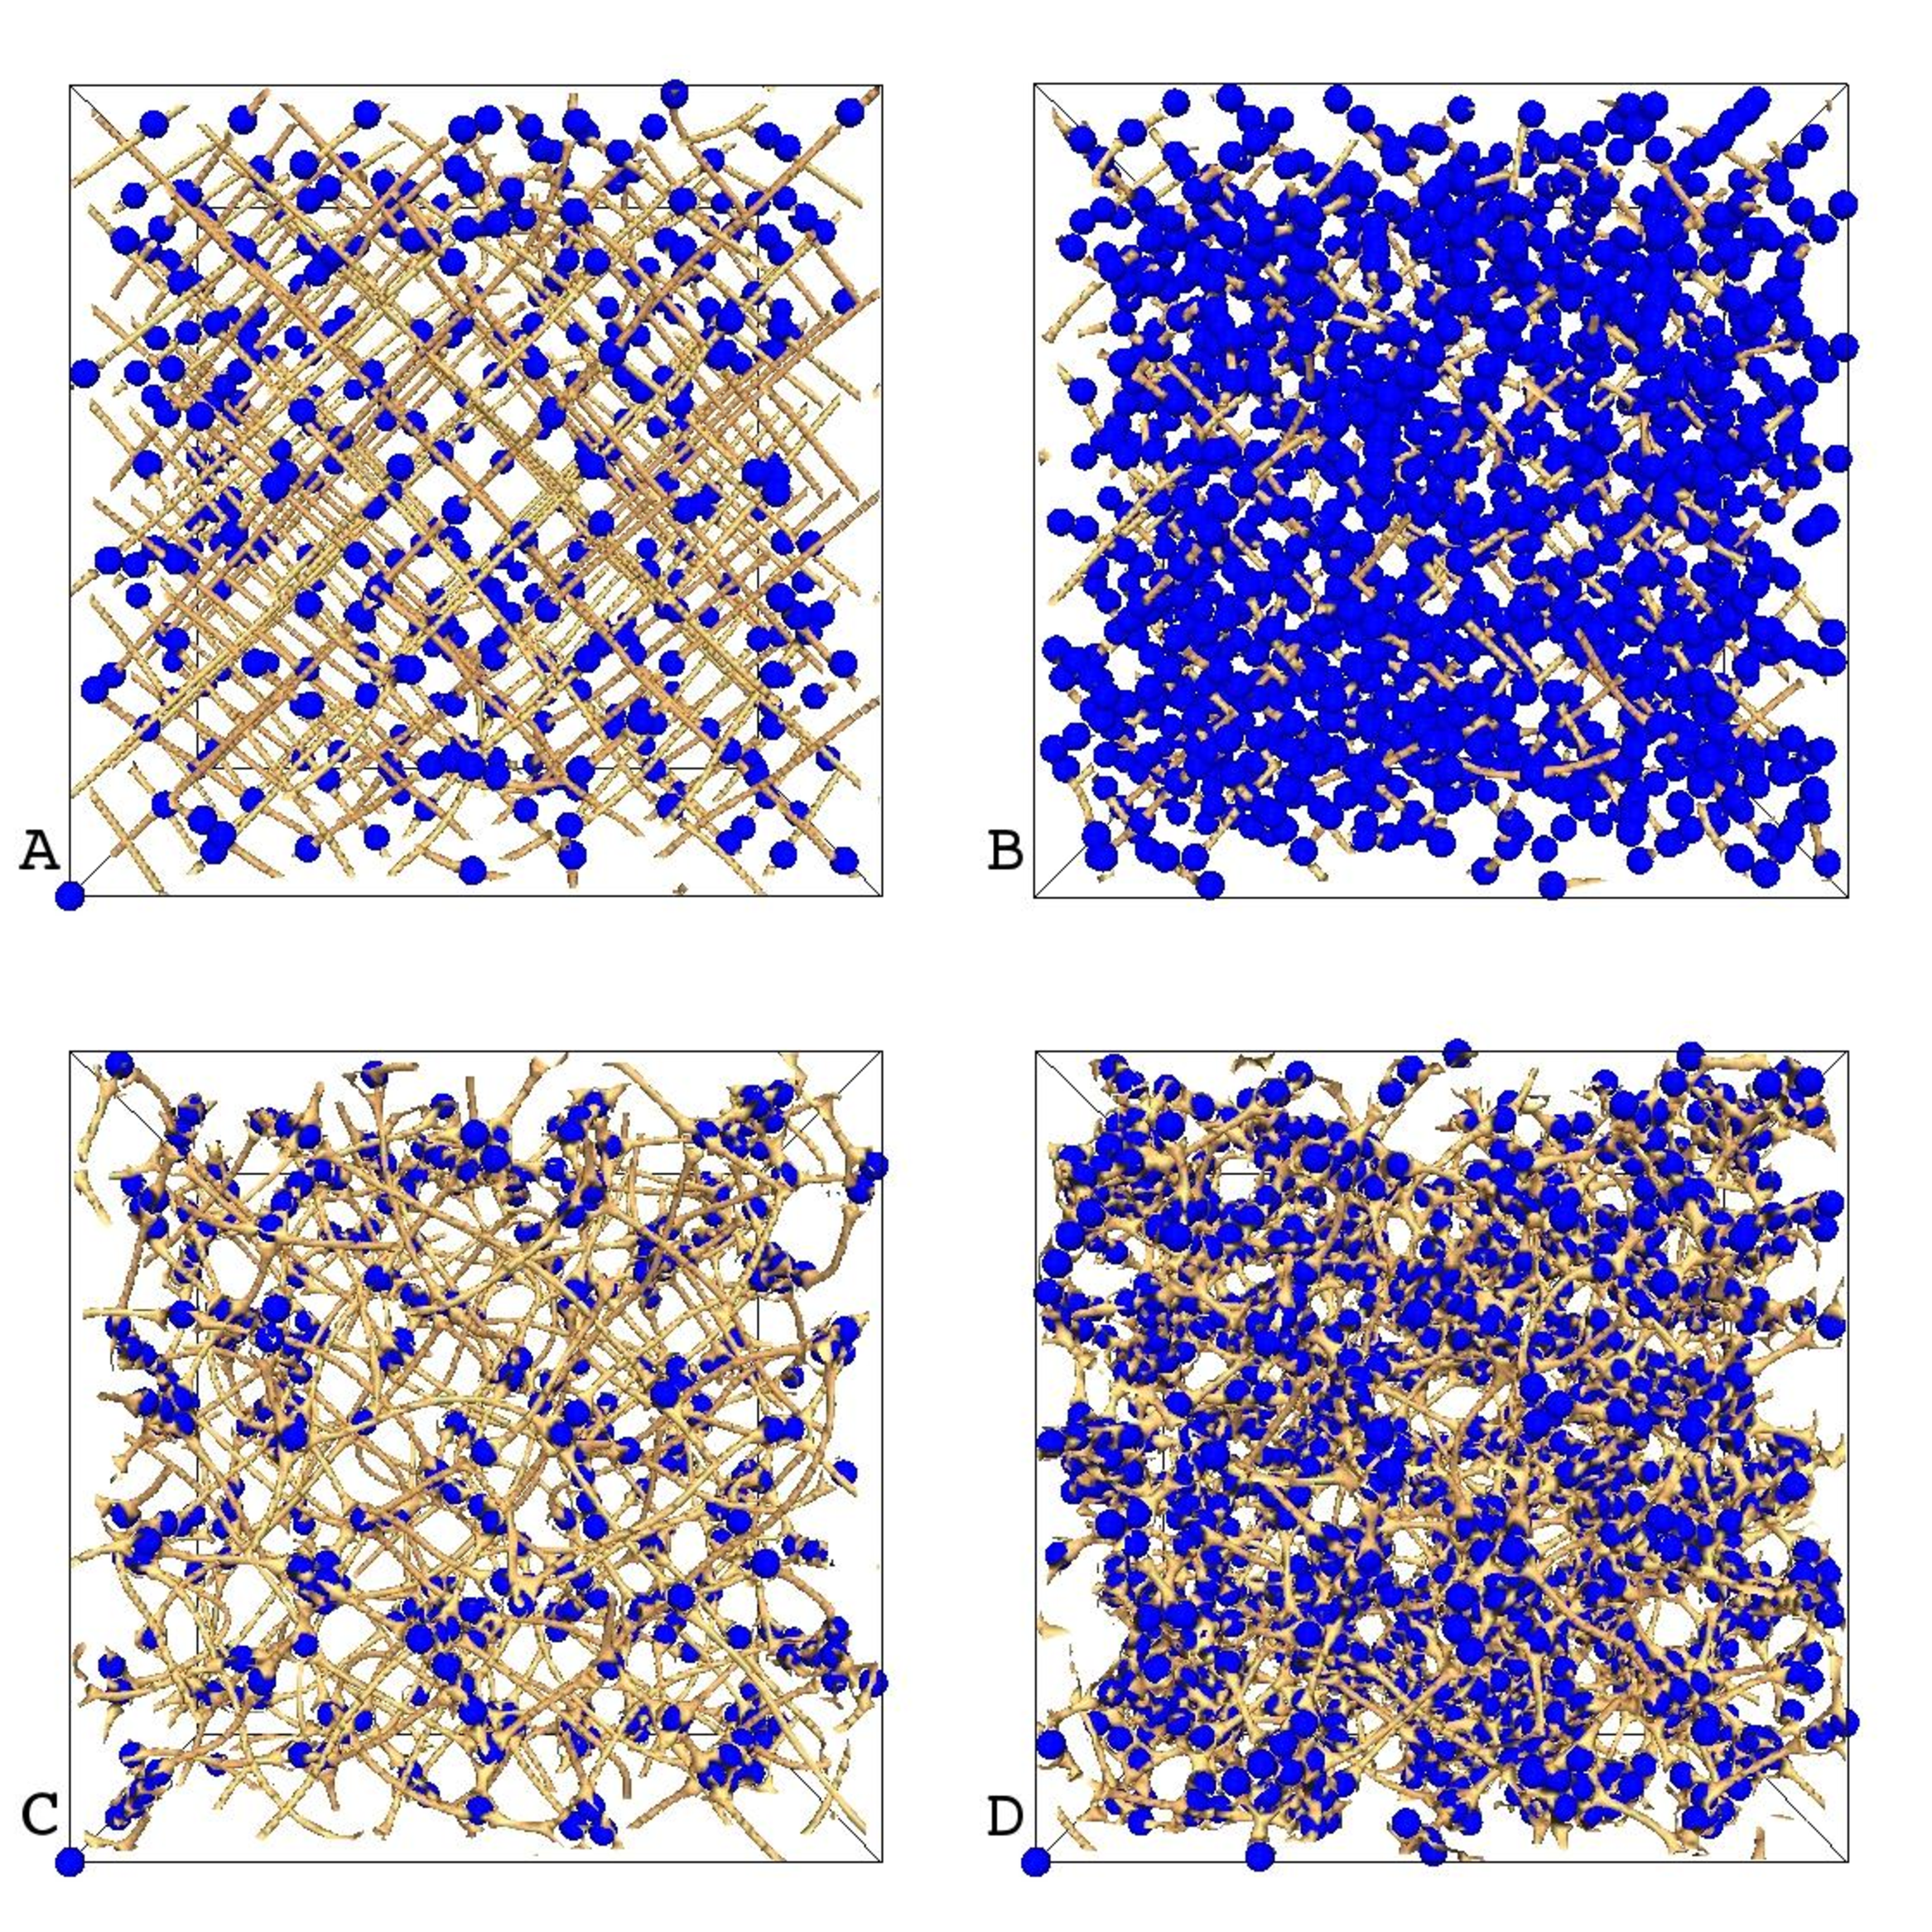
\includegraphics[scale=0.35]{support-fig2.pdf}
\end{center}
\caption{As for main manuscript Fig.~1 A--D
(with liquid crystal order parameter
initialised to equilibrium blue phase I structure), but for the entire
simulation system of 128$^3$ lattice sites. (A)  solid volume fraction~1\%
and weak anchoring;  (B) 4\% solid volume fraction and weak anchoring;
(C) 1\% solid volume fraction and strong anchoring; (D) 4\% solid
volume fraction and strong anchoring. The view direction in the
main figure is from the left here. There is a reference
particle at the bottom left in each panel which does not take part
in the simulation.}
\end{figure}

\newpage

\begin{figure}[!h]
\begin{center}
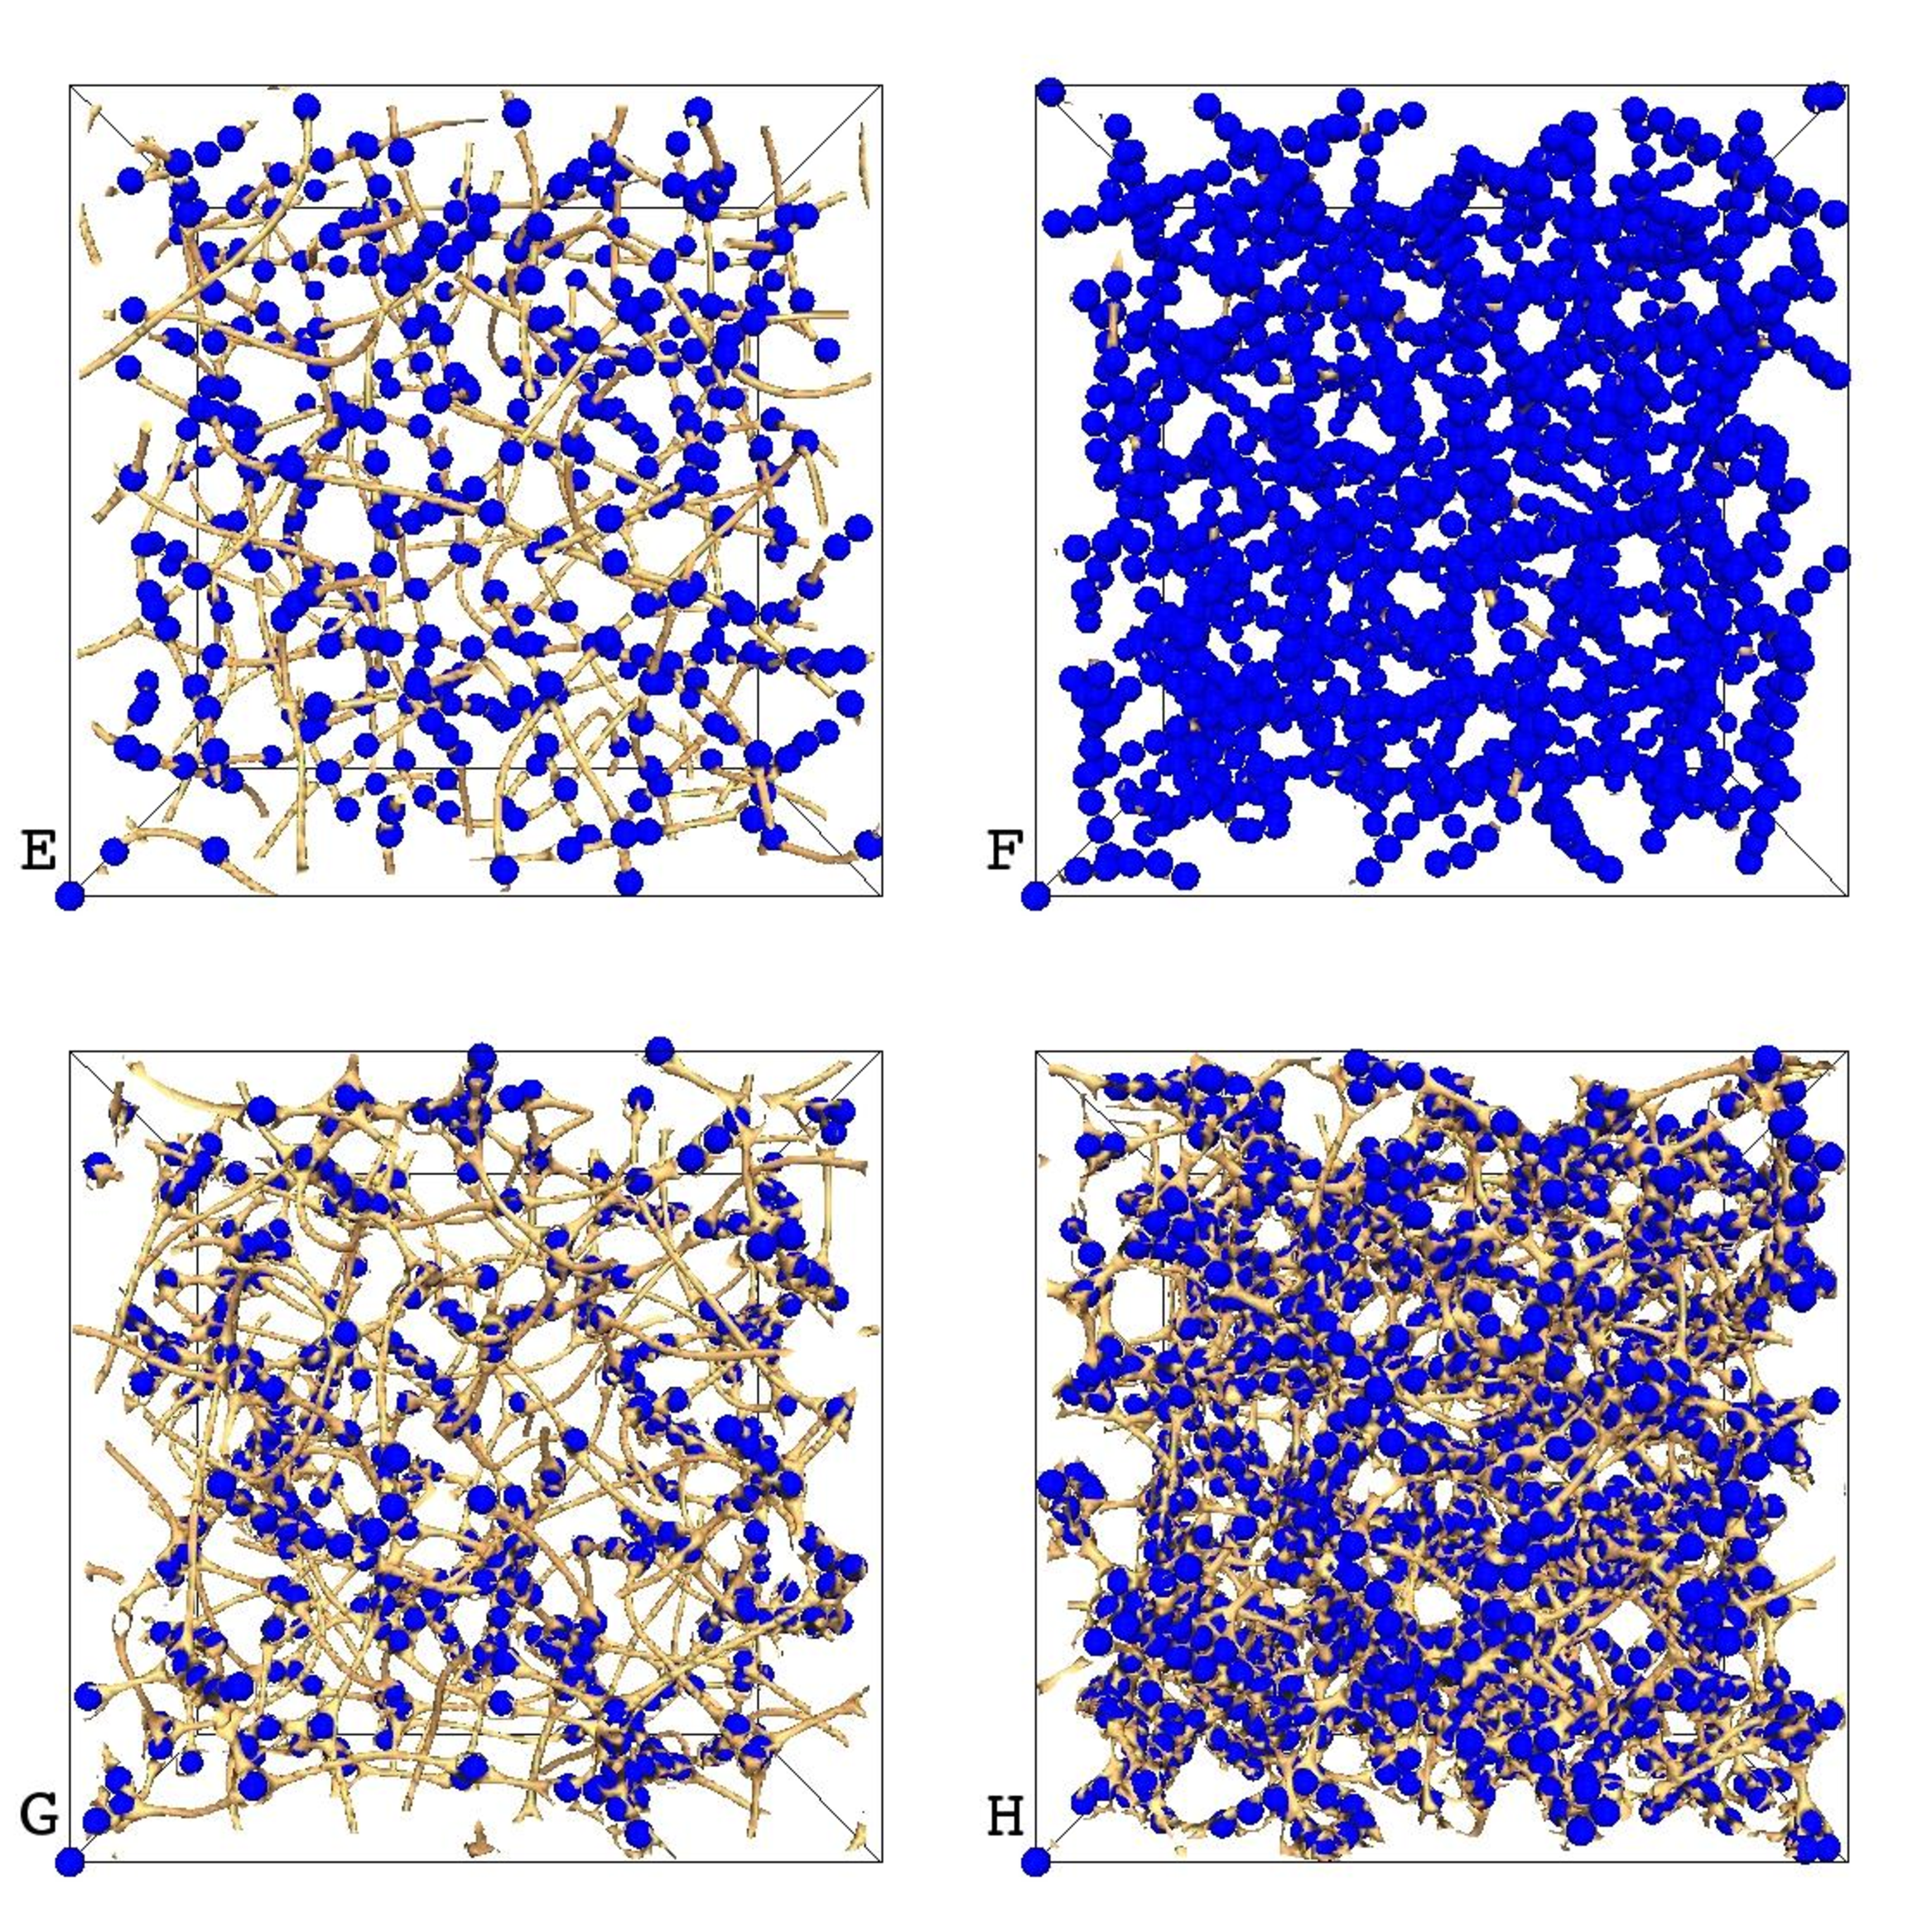
\includegraphics[scale=0.35]{support-fig3.pdf}
\end{center}
\caption{As for main manuscript Fig.~1 E--H (initialised via a ``quench''
to generate a disordered network), but for the entire simulation
system of 128$^3$ lattice sites. (E) solid volume fraction 1\% and
weak anchoring; (F) 4\% solid volume fraction and weak anchoring;
(G) 1\% solid volume fraction and strong anchoring; (H) 4\% solid
volume fraction and strong anchoring. Again, there is a reference
particle at the bottom left in each case which does not take part
in the simulation.}
\end{figure}

\newpage

\begin{figure}[!h]
\begin{center}
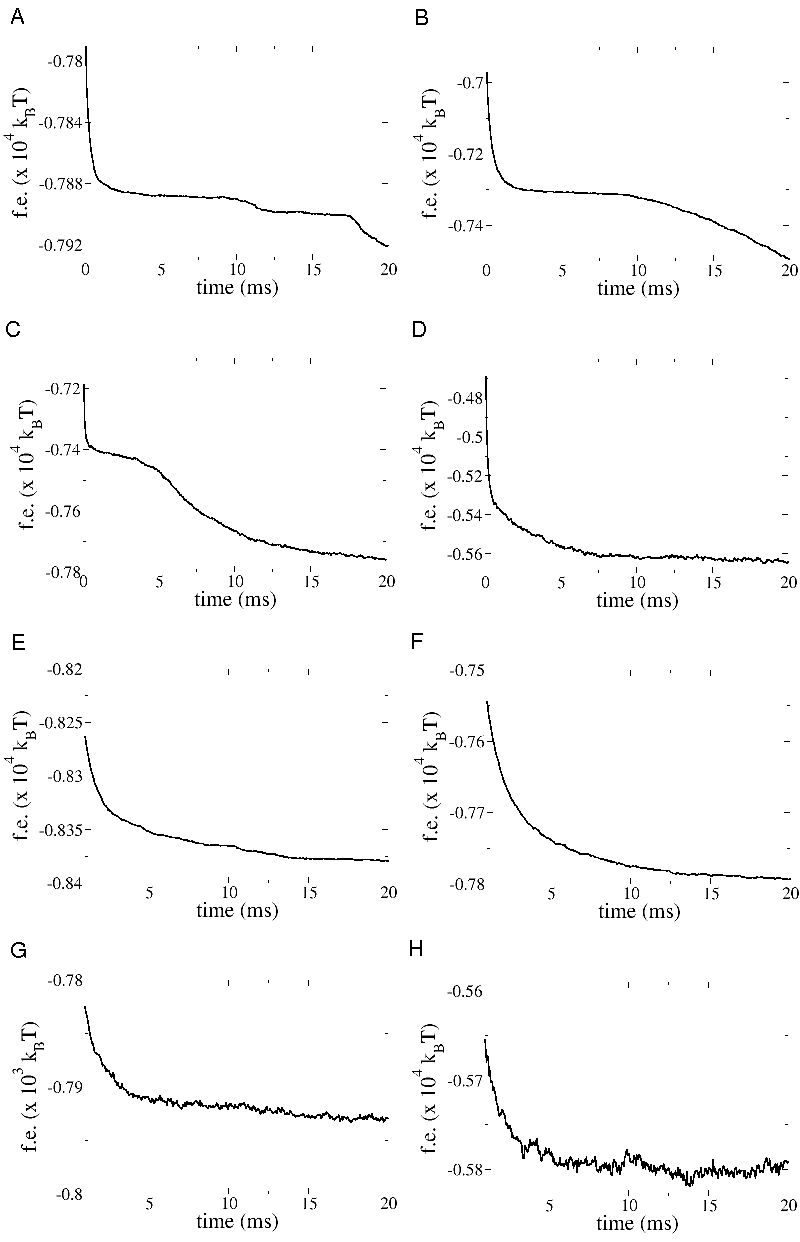
\includegraphics[scale=0.49]{support-fig4.png}
\end{center}
\caption{Plot of the free energy (per BP unit cell) versus time
for the simulations corresponding to Fig. 1A-H in the main text
(the labels correspond to those in Fig. 1).
}
\end{figure}

\newpage

\begin{figure}[!h]
\begin{center}
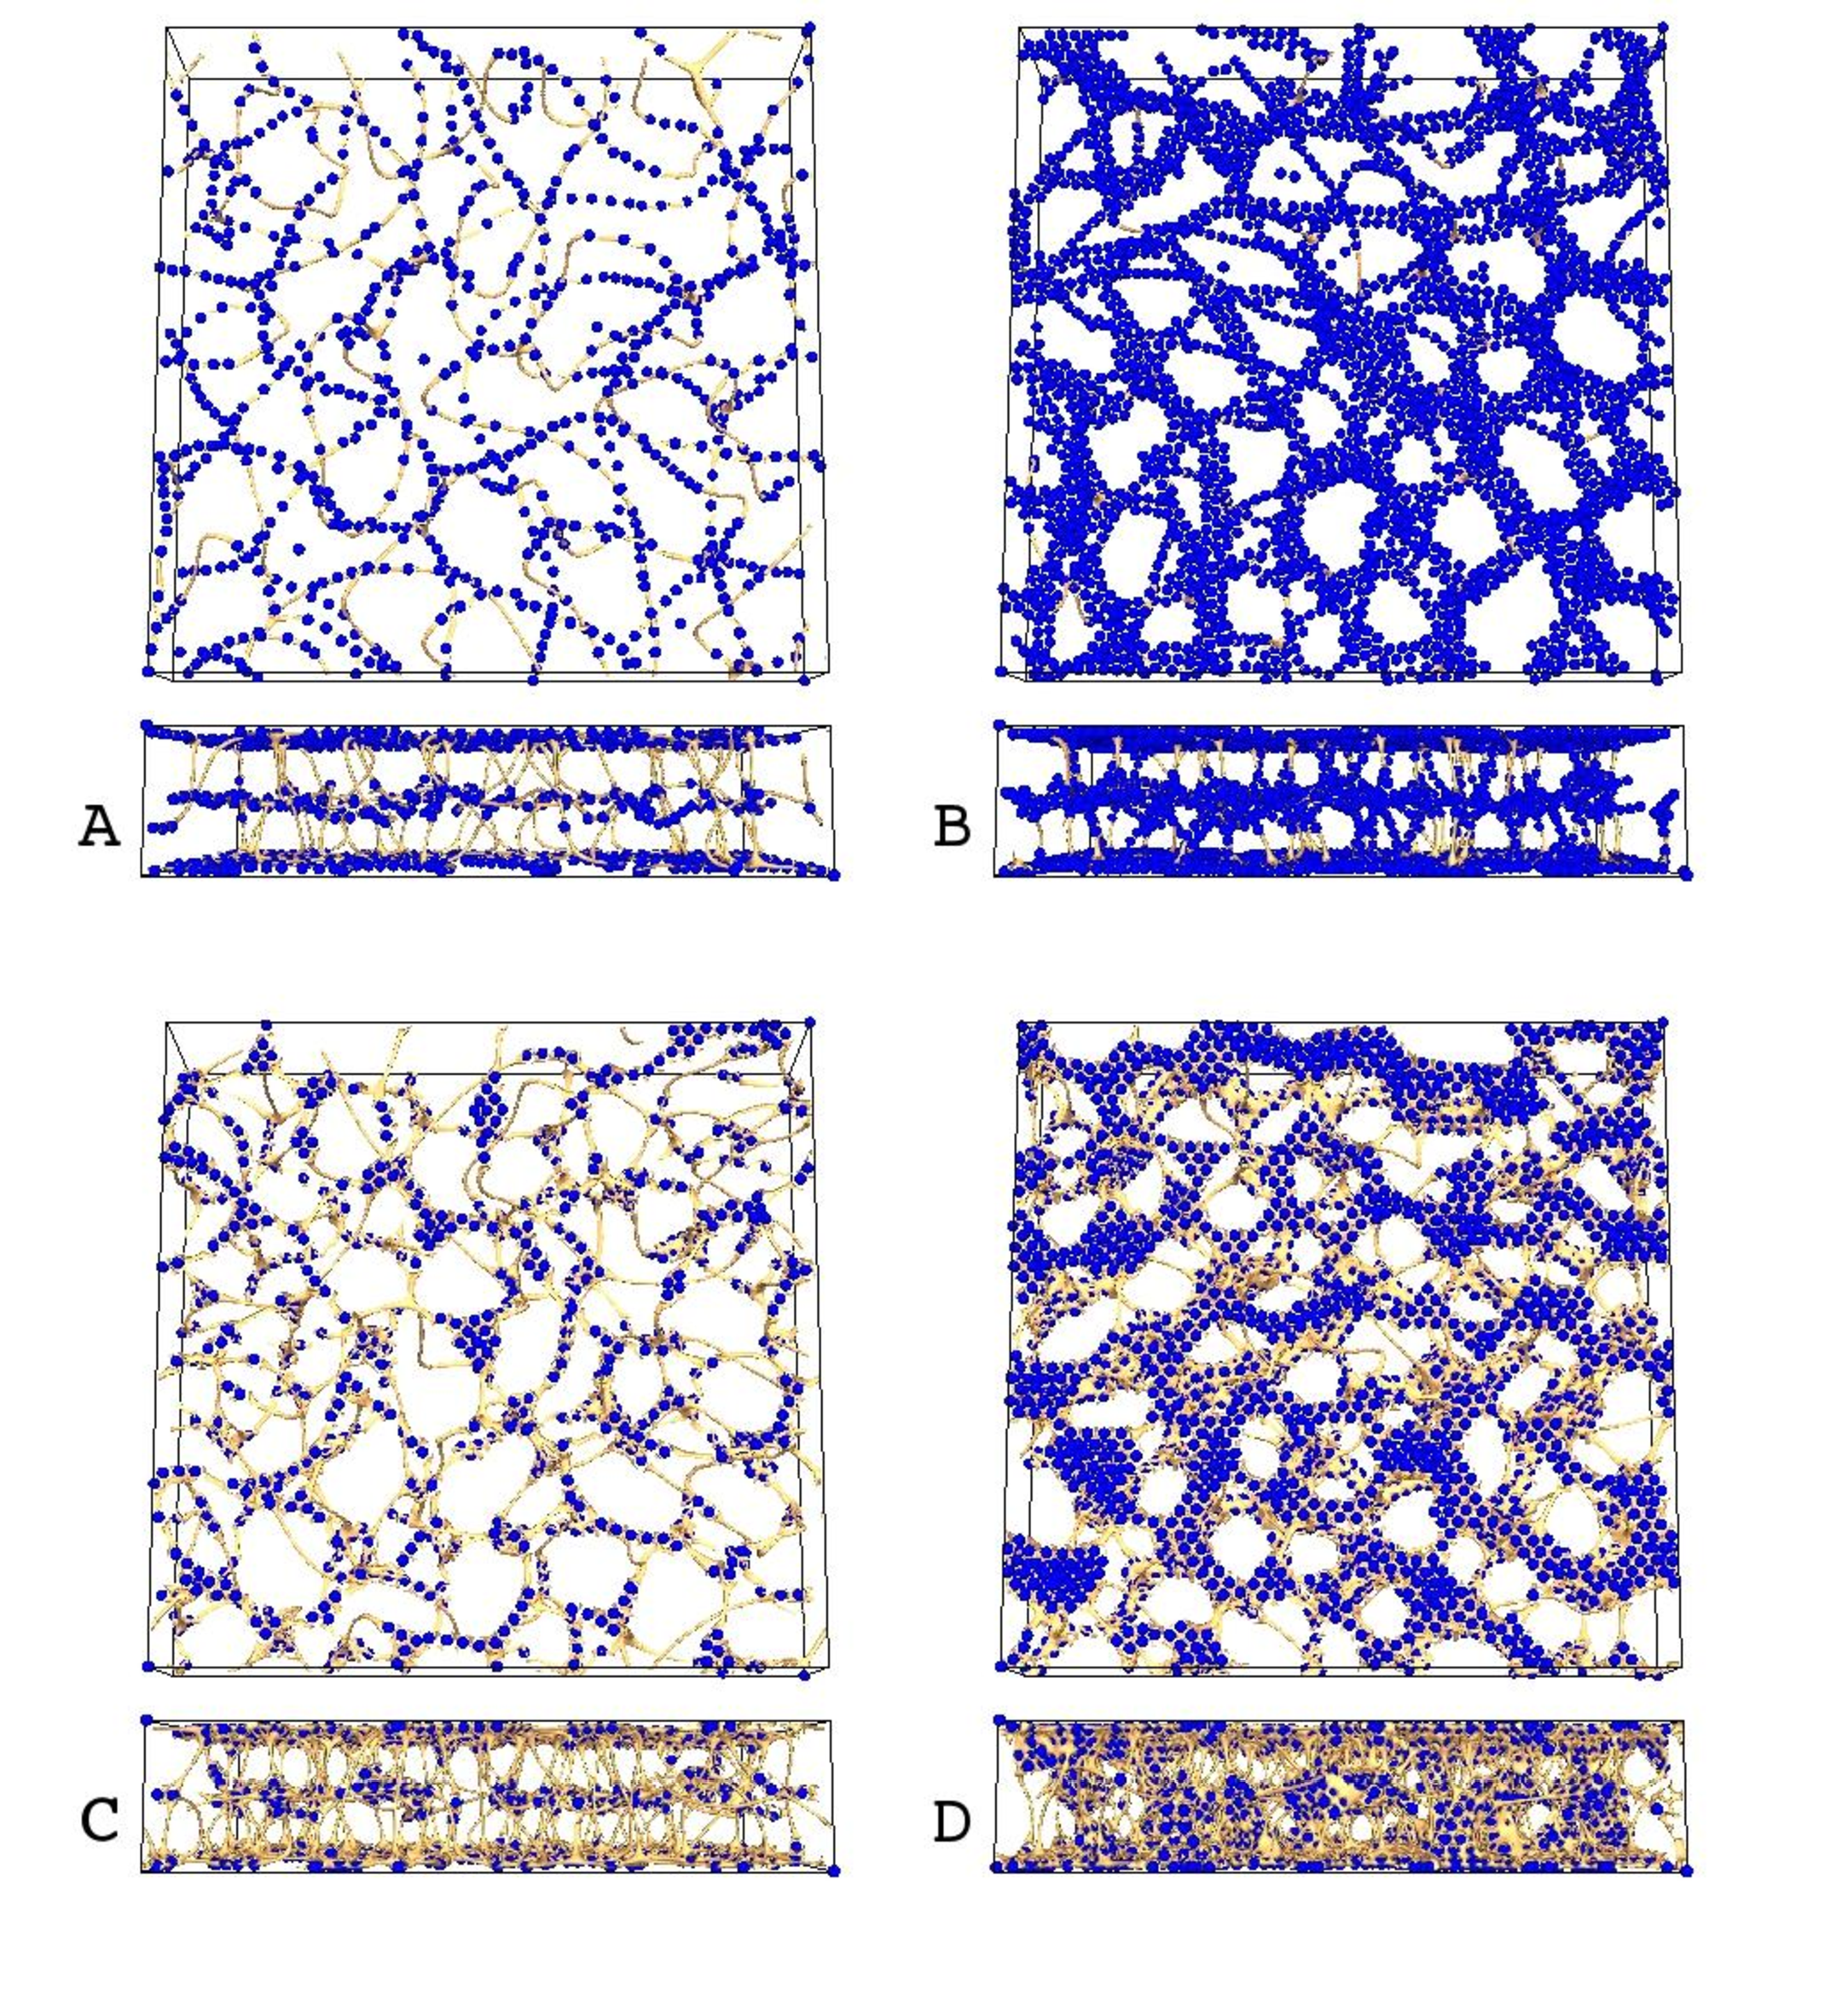
\includegraphics[scale=0.42]{support-fig5.pdf}
\end{center}
\caption{As for main manuscript Fig.~2 A--D (confined geometry with normal
anchoring walls at both top and bottom), but for the entire simulation
system of 256$^2\times$56 lattice sites. Each shows a top view and
side view of the same simulation state. (A) solid volume fraction 1\%
and weak anchoring; (B) 4\% solid volume fraction and weak anchoring;
(C) 1\% solid volume fraction and strong anchoring; (D) 4\% solid
volume fraction and strong anchoring.}
\end{figure}

\newpage

\begin{figure}[!h]
\begin{center}
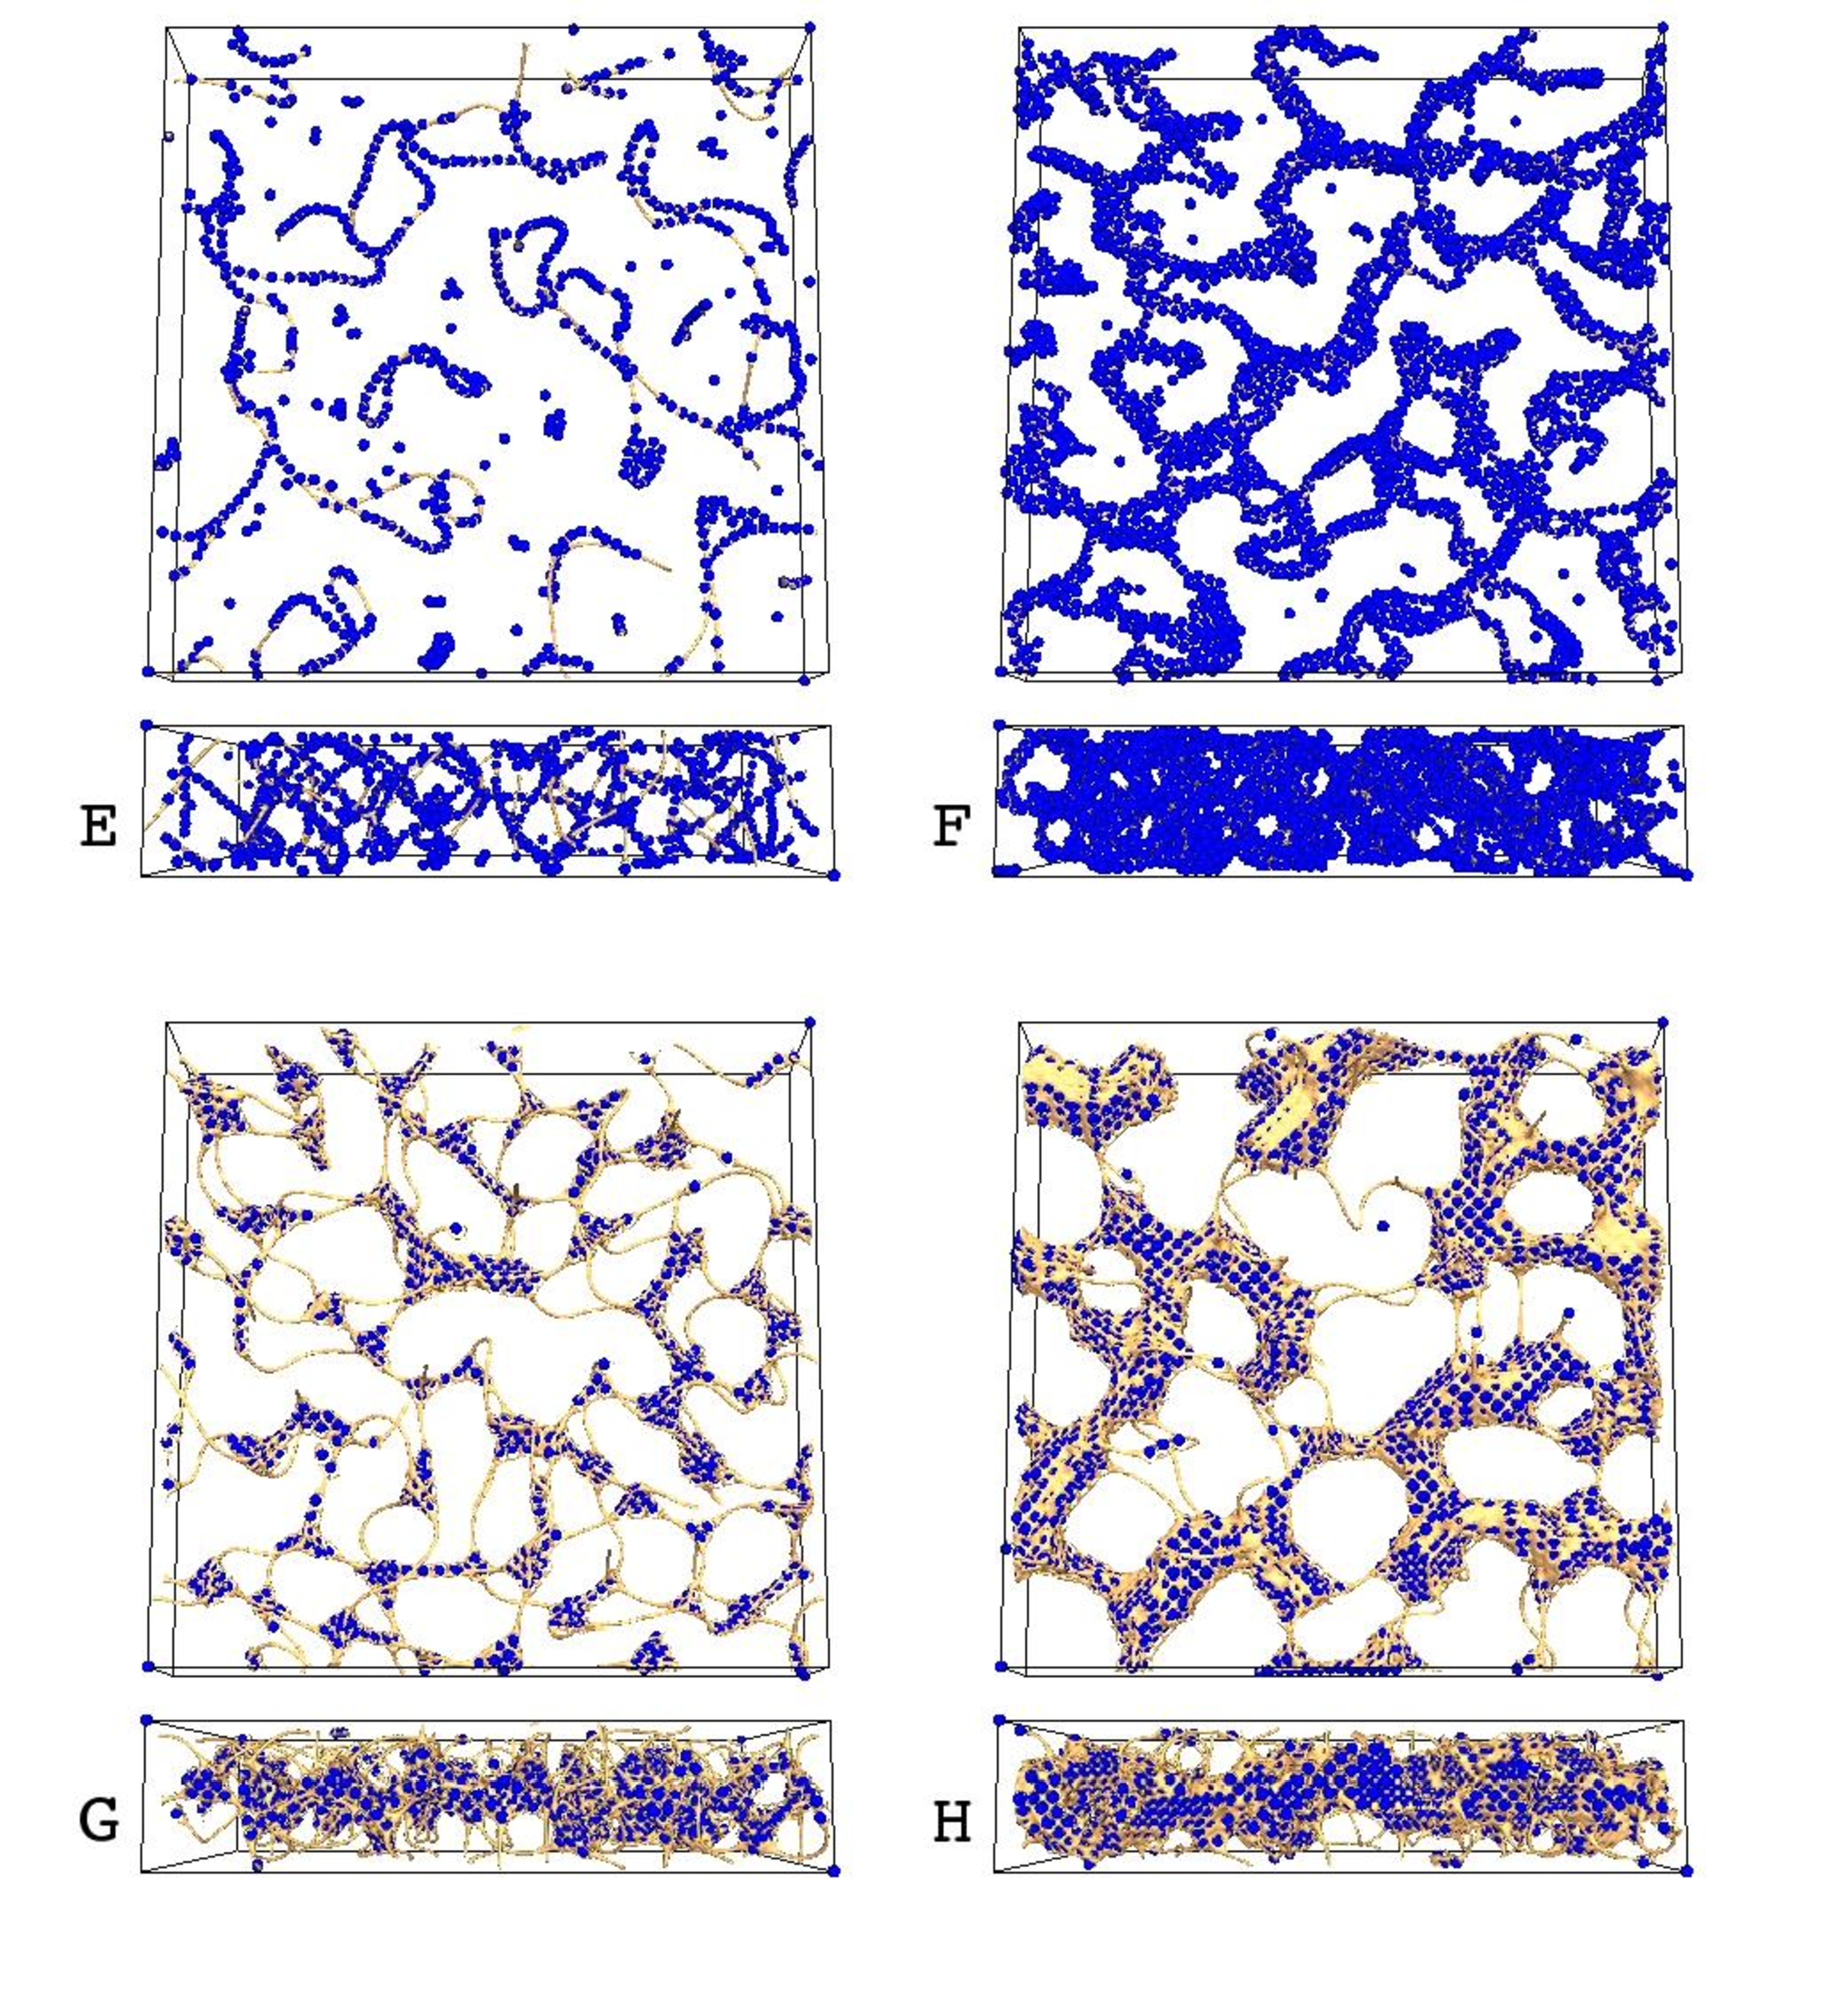
\includegraphics[scale=0.42]{support-fig6.pdf}
\end{center}
\caption{As for main manuscript Fig.~2 E--H (confined geometry with planar
anchoring walls at both top and bottom), but for the entire simulation
system of 256$^2\times$56 lattice sites. Each shows a top view and
side view of the same simulation state. (E) colloid solid volume fraction 1\%
and weak anchoring; (F) 4\% solid volume fraction and weak anchoring;
(G) 1\% solid volume fraction and strong anchoring; (H) 4\% solid
volume fraction and strong anchoring.}
\end{figure}

\newpage


\begin{figure}[!h]
\begin{center}
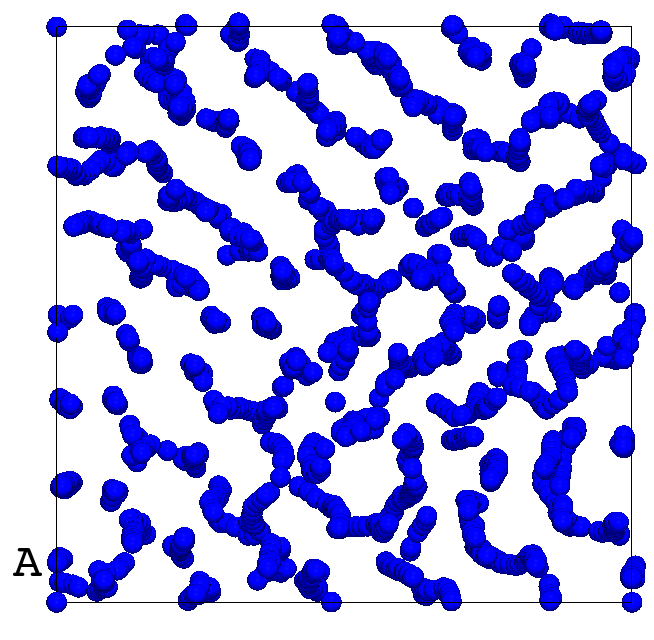
\includegraphics[width=0.32\columnwidth]{col_parallel_x_run1341.png}
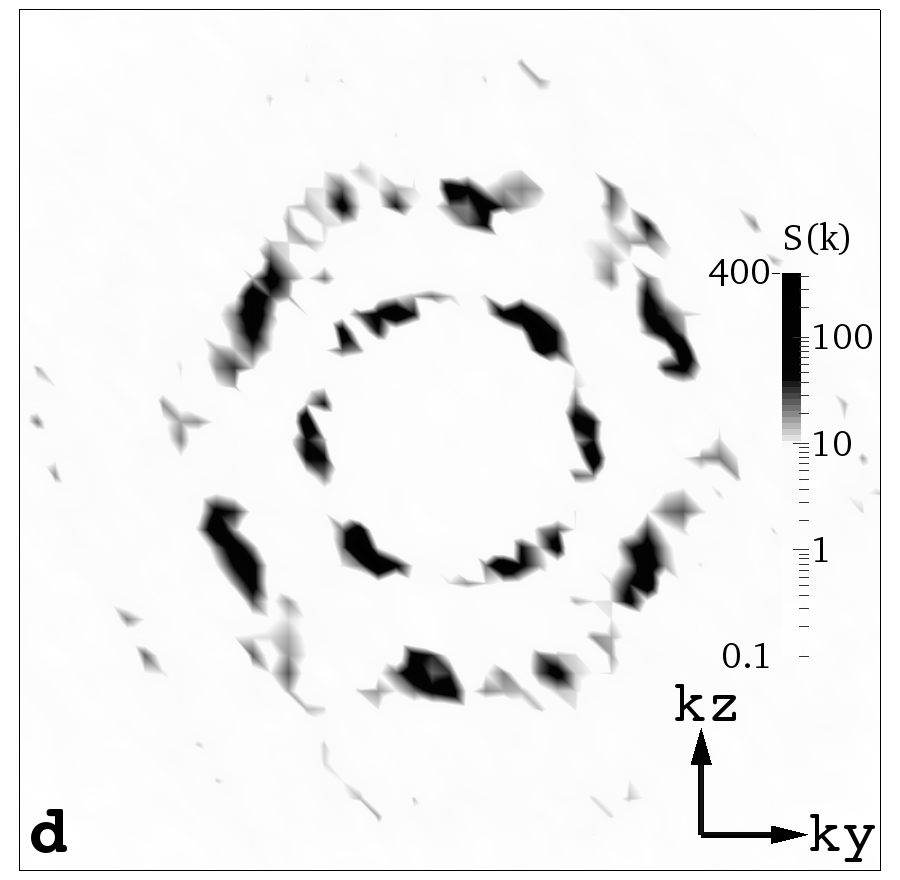
\includegraphics[width=0.32\columnwidth]{sq_x_run1341.png}
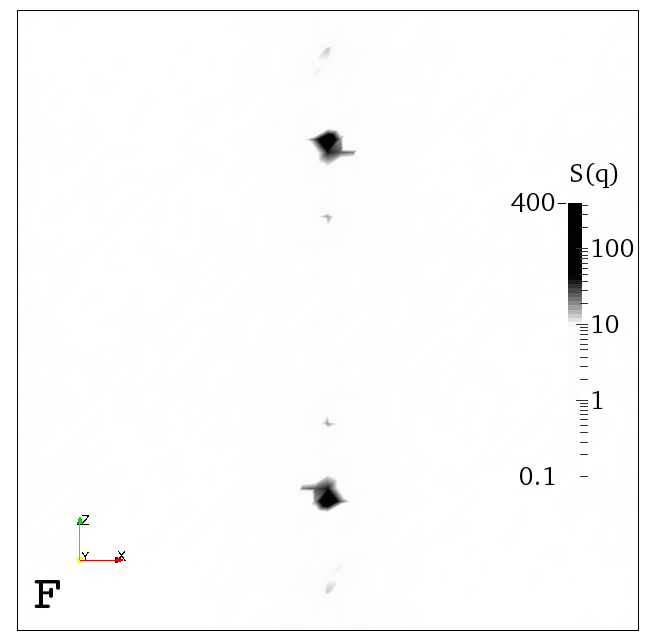
\includegraphics[width=0.32\columnwidth]{sq_y_run1341.png}
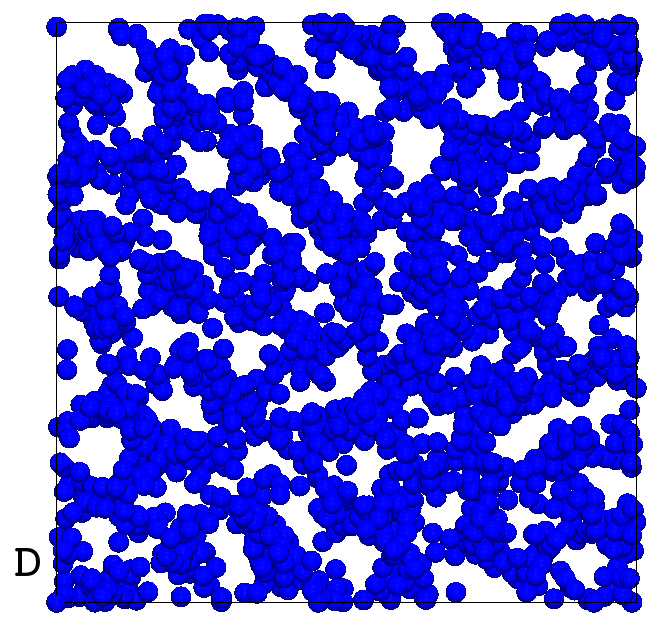
\includegraphics[width=0.32\columnwidth]{col_parallel_x_run1342.png}
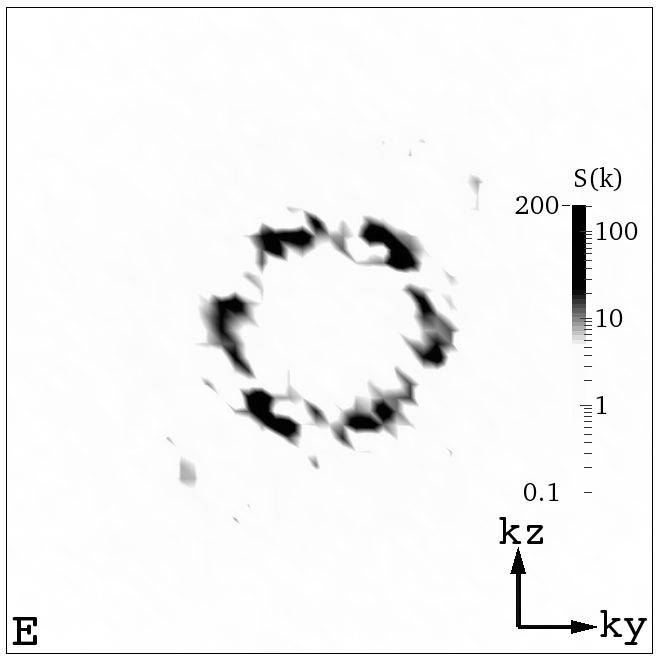
\includegraphics[width=0.32\columnwidth]{sq_x_run1342.png}
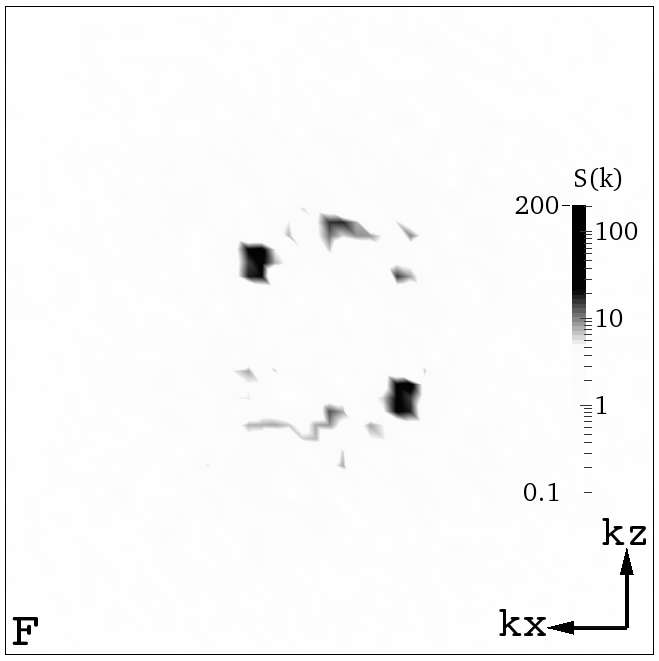
\includegraphics[width=0.32\columnwidth]{sq_y_run1342.png}
\end{center}
\caption{Structure with and without electric field, with disclination lines
removed for clarity. Panels A and B reproduce the results Fig. 3 panels
C and D with the applied field in the $x$-direction (into the plane of the
paper). Also included is a cut of the structure factor with $k_y = 0$
(panel C). Panels D, E, and F show the corresponding situation after the
external field has been removed and the structure allowed to relax,
and show residual hexagonal ordering. The structure factor data is for wave
vectors $k_x = 0; (k_y, k_z) \in [-3\pi/8 , 3\pi/8]$ (panels B and E) and
$k_y = 0; (k_x, k_z) \in [-3\pi/8, 3\pi/8]$ (panels C and F).
[ADD PARTICLE Y-VIEW?]}
\end{figure}

\newpage

\begin{figure}[!h]
\begin{center}
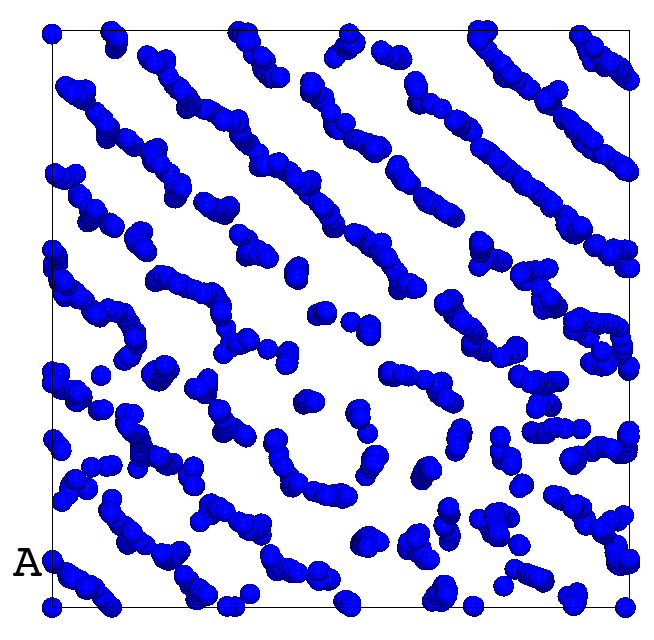
\includegraphics[width=0.32\columnwidth]{col_parallel_y_run1343.png}
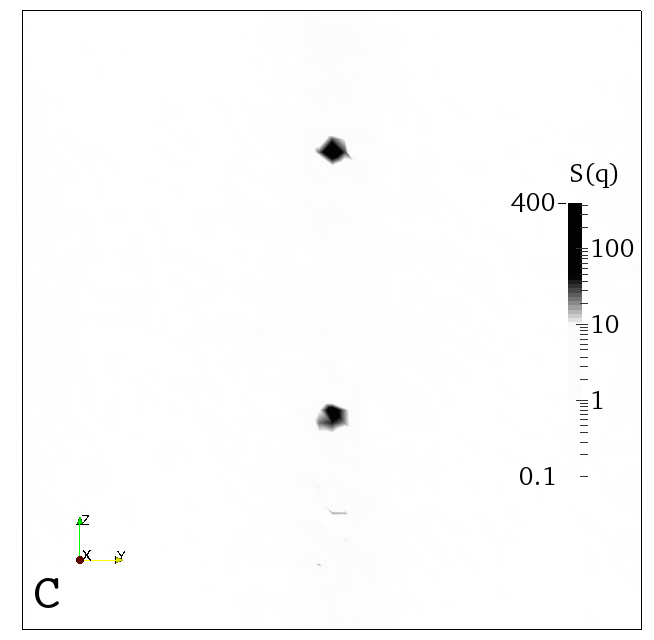
\includegraphics[width=0.32\columnwidth]{sq_x_run1343.png}
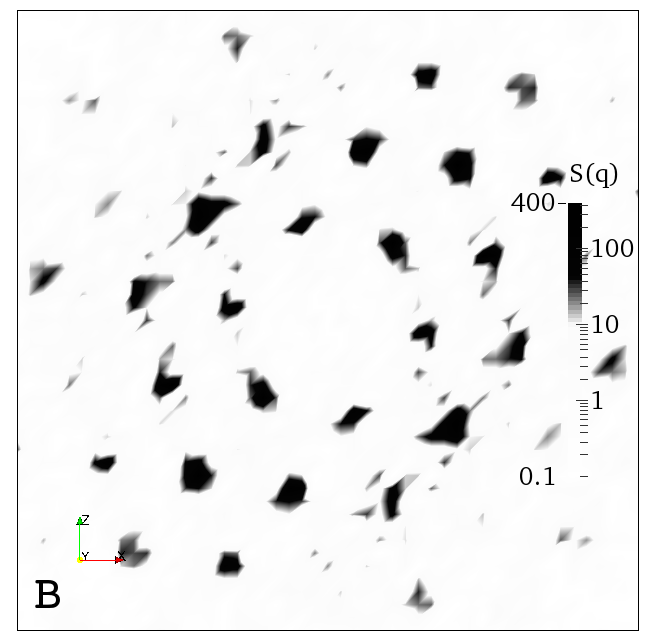
\includegraphics[width=0.32\columnwidth]{sq_y_run1343.png}\\
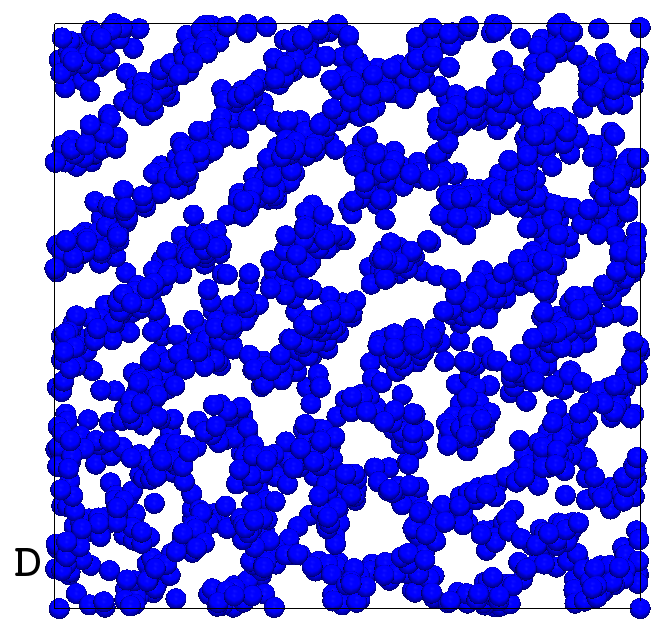
\includegraphics[width=0.32\columnwidth]{col_parallel_y_run1344.png}
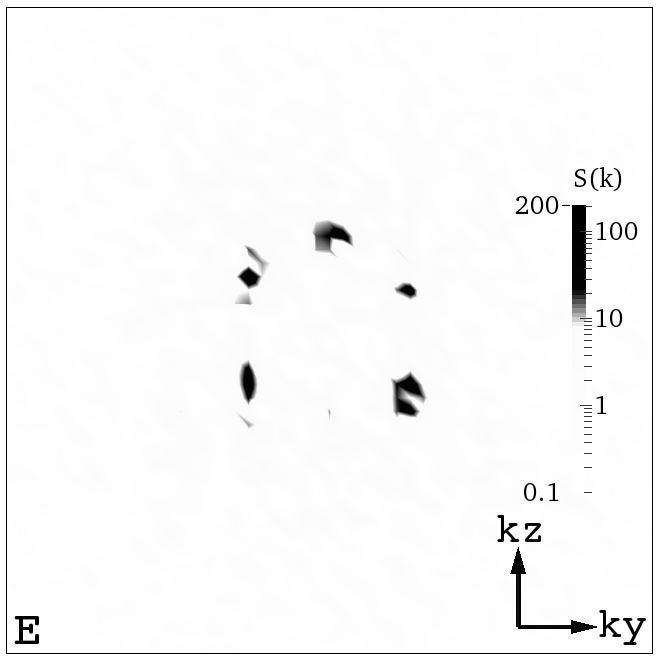
\includegraphics[width=0.32\columnwidth]{sq_x_run1344.png}
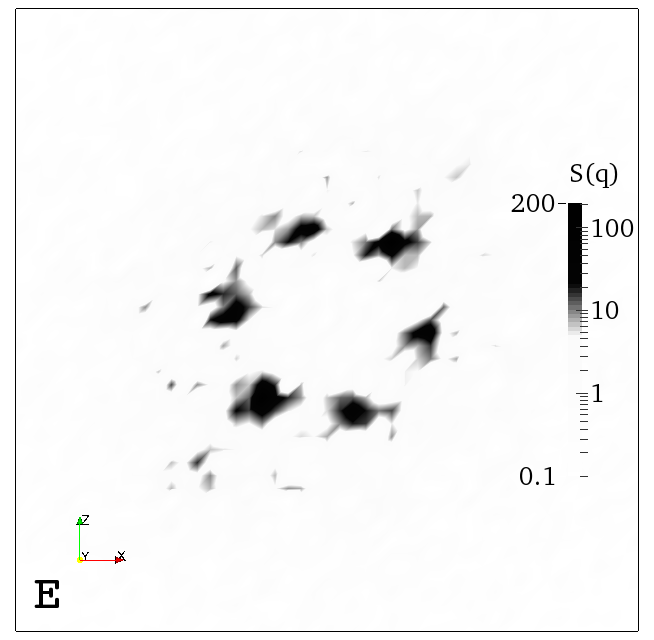
\includegraphics[width=0.32\columnwidth]{sq_y_run1344.png}\\
\end{center}
\caption{Cycling the electric field. Starting from the final position of
Supplementary Fig.~7 panel~C, the field is re-applied, this time in the
$y$-direction. The corresponding view of the particle distribution is
shown, again viewing along the field direction, in panel A.
Corresponding structure factor cuts with $k_x = 0$ and $k_y = 0$ are
shown in panels B and C, respectively. The corresponding situation when
the field is again switched off, and the structure allowed to relax,
is shown in panels d, E, and F. The wave vector values used are the
same as in Supplementary Fig.~7. [ADD PARTIVLE $y$-VIEW?]}
\end{figure}

\newpage

\begin{figure}[!h]
\begin{center}
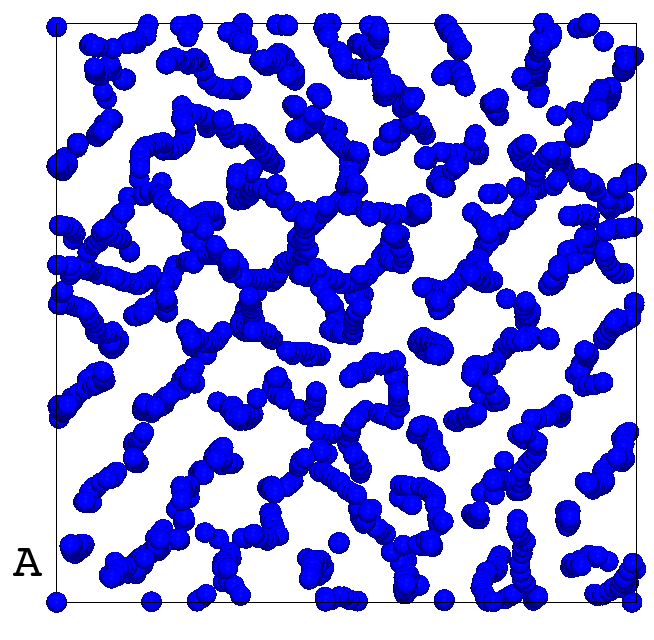
\includegraphics[width=0.32\columnwidth]{col_parallel_x_run1345.png}
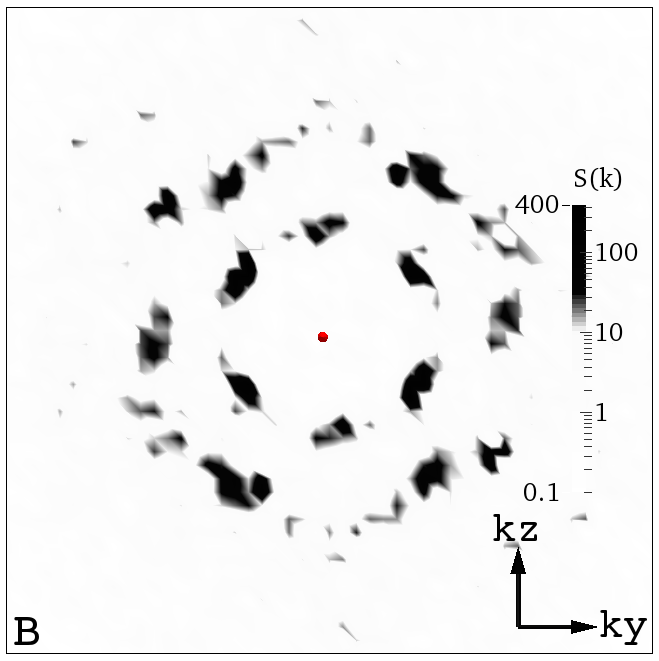
\includegraphics[width=0.32\columnwidth]{sq_x_run1345.png}
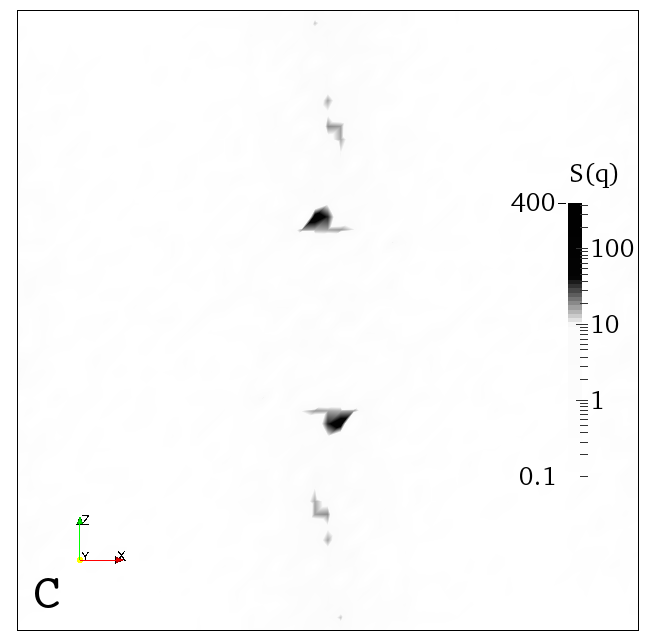
\includegraphics[width=0.32\columnwidth]{sq_y_run1345.png}\\
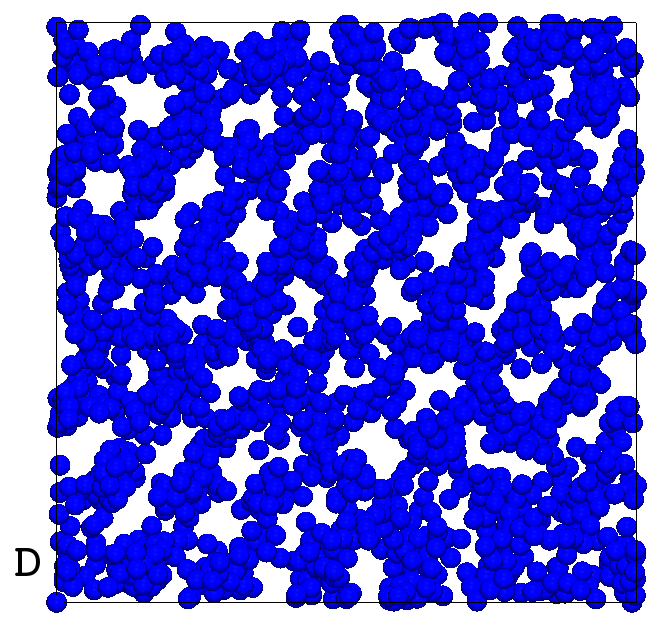
\includegraphics[width=0.32\columnwidth]{col_parallel_x_run1347.png}
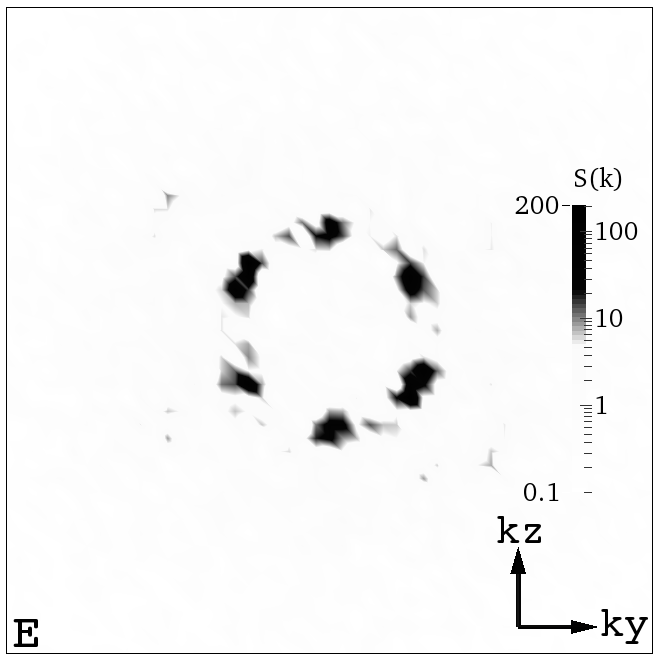
\includegraphics[width=0.32\columnwidth]{sq_x_run1347.png}
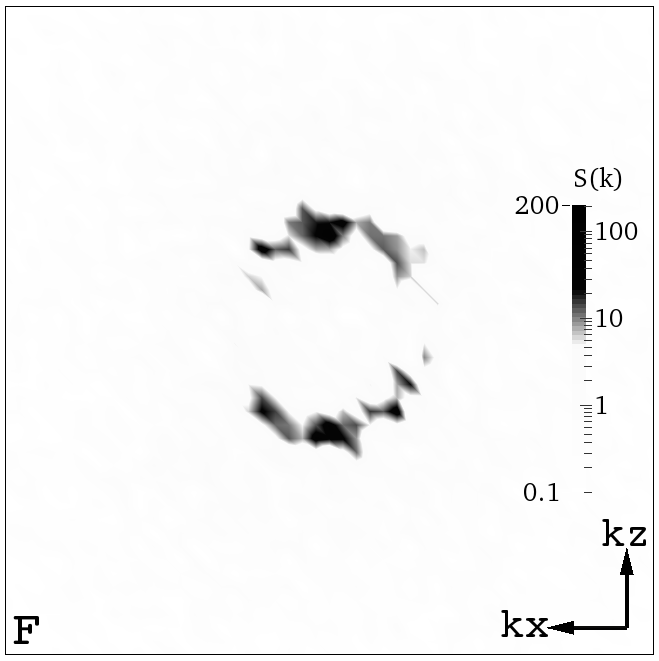
\includegraphics[width=0.32\columnwidth]{sq_y_run1347.png}
\end{center}
\caption{Cycling the electric field further. Starting from the final
position of Supplementary Fig.~8 panel~D, the field is re-applied
again in the $x-$direction. Panel A shows the particle configuration
viewed along the field direction, and panels B and C show the structure
factor with $k_x = 0$ and $k_y = 0$ respectively. The corresponding
situation when the field is removed and the structure allowed to relax
is shown in panels D, E, and F. The wave vector values are again as
in Supplementary Fig.~7. [DIFFERENCE CF 7?]}
\end{figure}

%\newpage
\clearpage
 
{\bf Captions for Supplementary Movies} \\

{\bf Supplementary Movie 1:} 
The final state of the simulation as shown in Fig.~1A. The movie
rotates the configuration to reveal more clearly its structure.\\

{\bf Supplementary Movie 2:} 
The final state of the simulation as shown in Fig.~1B. The movie
rotates the configuration to reveal more clearly its structure.\\


{\bf Supplementary Movie 3:} 
The final state of the simulation as shown in Fig.~1C. The movie
rotates the configuration to reveal more clearly its structure.\\


{\bf Supplementary Movie 4:} 
The final state of the simulation as shown in Fig.~1D. The movie
rotates the configuration to reveal more clearly its structure.\\


{\bf Supplementary Movie 5:} 
The configuration after the initial relaxation phase in Fig.~3. The movie
shows a rotation of the configuration. The distribution of the colloidal
particles is isotropic, with the particles forming clusters and having a
tendency to occupy positions at the intersection of the BPIII disclination
lines.\\

{\bf Supplementary Movie 6:} 
Configuration in a homogeneous electric field with strength
corresponding to ${\cal E}=0.8$. The movie
shows a rotation of the configuration.
A hexagonal pattern emerges where the particles form chains
situated at the vertices of the honeycomb-like structure. \\

\end{document}
